%\documentclass[]{article}
\documentclass[]{elsarticle}
\usepackage{amsmath}
%\usepackage{cite}
\usepackage{bm}
\usepackage{color}
\usepackage{amssymb}
\usepackage{graphicx}
\usepackage{epstopdf}
%\usepackage[margin=1in]{geometry}
\usepackage{caption}
\usepackage{subcaption}
\usepackage{multirow}
\usepackage{color}
\usepackage{xcolor}
\usepackage[final]{pdfpages}
\usepackage{lineno}
\modulolinenumbers[5]

%%%so that figures appear in their section
\usepackage[section]{placeins}

%%%% SYMBOLS
\renewcommand{\vec}[1]{\mathbf{#1}}

\begin{document}


\linenumbers

\section*{Introduction}
The textwidht for this paper is : \the\textwidth


To compile the code
\begin{verbatim}
cmake .
make
\end{verbatim}

To generate the measurements
\begin{verbatim}
./data gcase00.cfg
\end{verbatim}

To run the static parameter case
\begin{verbatim}
mpirun -np 12 ./run case00.cfg
\end{verbatim}


To run the time-varying parameter case
\begin{verbatim}
mpirun -np 10 ./run case00b.cfg
mpirun -np 10 ./run case00c.cfg
mpirun -np 10 ./run case00d.cfg
mpirun -np 10 ./run case00e.cfg
mpirun -np 10 ./run case00f.cfg
\end{verbatim}
To display the results (eps figures will be saved in the figs folder)
\begin{verbatim}
python draw.py
\end{verbatim}

\subsection*{Configuration files}
The various parameters can be changed in different files.
In the file "functions.cpp", the models are coded. In the ".cfg" files, the parameters for each cases are present. The file "gcase00.cfg" controls data generation. The important parameters are
\begin{verbatim}
	name 			= 	"First Order SDE (colored noise!)";
	handle 			=	"FirstOrder";
	folder			=	"Case00";
	initialState 	=	[1.0];
	parameters			=	[1.0, 0.01];
	time			=	10.0;
	dt				=	0.001;
	stepsBetweenMeasurements = 10;
	NSR				=	0.25;
\end{verbatim}
where handle corresponds to the function in "functions.cpp". The {\bf folder} "Case00" is where the measurements will be stored. The initial state of the system is $x = 1.0$ ( {\bf initialState}). The parameter vector $[1.0, 0.01]$ corresponds to $[\alpha, \sigma]$. The keyword {\bf time} controls for how long is the system simulated, {\bf dt} is the timestep, {\bf stepsBetweenMeasurements} controls how many time steps between each measurements and {\bf NSR} is the noise to signal ratio.

The other configuration files control the parameter and state estimation problem. In "case00.cfg" the following can be found
\begin{verbatim}
folder																=	"Case00";
dt																		=	0.001;
fStepsBetweenMeasurements 						=	10;
measurementCov												=	"variance.dat";
data																	=	"data.dat";
Parameter_Estimation 									= true;
Evidence_Estimation 									= false;
State_Estimation											= false;
seruns 																= 1;
\end{verbatim}
Where {\bf folder} specifies where the measurements can bve found, {\bf data} and { \bf measurementCov} are the name of the files where measurements and the measurement variance are stored.  The true and false indicates that parameter estimation is performed but stand alone state estimation is not performed. The state estimation procedure included in the parameter estimation problem is still performed. For each proposed models we have the following configuration keywords

\begin{verbatim}
	run							=	true;
	name 						=	"StaticParameters";
	state_estimator				=	"ekf";
	handle 						=	"m2";
	initialState 				=	[5.0];
	nprocs						= 1;
	initialStateVariance 		= ([0.1])
	//parameters 				= (0.2, 0.1);
	prior					= 	(
		"Uniform", 0.0, 10.0,
		"Uniform", 0.0, 10.0
	);
	parallelGroups				= 8;
	MCMC_CONFIG						=	{
		Method = "TMCMC";
		dim = 2;
		window = 40000;
		};
\end{verbatim}

{\bf run} controls wether this model will be run of not. The keyword {\bf state\_estimator} controls what filter is used for state estimation. The {\bf handle} links to the statespace created in "functions.cpp". {\bf initialState} and {\bf initialStateVariance} are the initial mean and covariance of the state. We use TMCMC to sample the posterior distribution. The dimension of the pdf is {\bf dim} $=2$ and there are window samples divided into 8 {\bf parallelGroups}. Each core is responsible for a group. {\bf nprocs} and {\bf parameters} are not used here.


The other configuration files control the state estimation procedure when the state is augmented. There could only be one configuration file but they are separated for convenience. For example, in case00d.cfg the following can be found
\begin{verbatim}
	run										= true;
	name 									=	"TimeVaryingParametersEnkfD";
	state_estimator				=	"enkfmpi";
	handle 								=	"m1enkf";
	initialState 					=	[1.0, 5.0];
	nparticles							=	10000;
	nprocs								=	4;
	initialStateVariance 	= ([0.1, 0.0],[0.0, 0.000001])
	parameters 						= (0.01,0.01);
\end{verbatim}
The statespace used is m1enkf defined in functions.cpp. The filter used is the parallel Enkf ({\bf state\_estimator} = "enkfmpi") the initial state is controlled by {\bf initialState}. The filter uses 4 processsors ({\bf nprocs}) and is composed of 10000 particles ({\bf nparticles}). The initial state variance ({\bf initialStateVariance}) is 
\begin{equation}
P_0 = \begin{bmatrix}
0.1 & 0 \\
0 & 0.000001
\end{bmatrix}
\end{equation}
and the parameters for $[\sigma, \gamma]$ are defined by {\bf parameters}. These can be changed as well.


\section*{Introduction}

We are looking at the estimation of parameters in the model or measurement operator that suddenly changes. Two examples will be covered. In the first case, a linear mass-spring-damper (MSD) system is simulated. The effective stiffness, damping and strength of model error is estimated. The MSD is held by two spring in parallel. At time $t_s$ a spring breaks and the effective stiffness of the system changes. Multiple approaches to estimate the parameters will be changed. 

In the second scenario, the spring doesn't break but the position sensor is faulty at time $t_s$. 


Rationale:
Underwater acoustic sensor
health monitoring

\section*{Theory}

This section contains a description of the bayesian algorithm for parameter estimation. Parameters can be described as static or as time-varying. Consider a model described by
\begin{equation}
\vec{X}_{k+1} = \vec{g}_k(\vec{X}_k, \vec{\Phi})
\end{equation}
The parameter vector $\vec{\Phi}$ can be described by $\left\lbrace  \vec{\Phi}_s, \vec{\Phi}_t \right\rbrace$ where $\vec{\Phi}_s$ is the vector of static parameters and $\vec{\Phi}_t$. Both parameters need to be estimated using sensor data. To estimate the static parameters, a MCMC procedure is used. Consider the model $\mathcal{M}$ having the unknown parameters $\vec{\Phi}_s$, the estimated values of the parameter after assimilating measurements is
\begin{align}
p(\vec{\Phi}_s | \vec{D}, \mathcal{M}) &= \frac{p(\vec{D} | \vec{\Phi}_s, \mathcal{M}) p( \vec{\Phi}_s | \mathcal{M})}{p(\vec{D} | \mathcal{M})} \\
&= frac{  \prod_{j=1}^J p(\vec{d}_j | \vec{\Phi}_s, \mathcal{M}) p( \vec{\Phi}_s | \mathcal{M})}{p(\vec{D} | \mathcal{M})}
\end{align}

 Bayesian inference provides a robust mathematical framework to combine measurements with model predictions. Sensor data is characterized by the following measurement equation~\cite{Evensen2009,jazwinski1970stochastic,prob}
\begin{equation}
 \vec{d}_{j} = \vec{h}_{j} (\vec{x}_{d(j)}, \vec{\varepsilon}_{j}) \label{eq:meas}
\end{equation}
where $\vec{d}_{j}$ is the observation vector at time step $t_{d(j)}$ and $\vec{\varepsilon}_j$ is the measurement noise modeled as a zero-mean Gaussian white noise process with known covariance.

The parameter likelihood can be expressed in terms of the state $\vec{x}$ vector.

\begin{equation}
p(\vec{d}_j | \vec{\Phi}_s, \mathcal{M}) = \int\limits_{-\infty}^{\infty} p( \vec{x}_{d(j)} | \vec{x}_{d(j)-1}, \vec{\Phi}_s) p(\vec{d}_j | \vec{x}_{d(j)} , \vec{\phi}_s) d \vec{x}_{d(j)}
\end{equation}

Bayesian model selection ranks the models based on the trade-off described in Eq.~\eqref{eq:evdatafiteig} between how well a model fits the data and its complexity. As seen in Eqs.~\eqref{eq:evidence_with_param} and ~\eqref{eq:evdatafiteig}, the evidence introduces the model parameters $\vec{\phi}$ where $p(\vec{D} |\vec{\phi},\mathcal{M}_i)$ is the likelihood, $p(\vec{\phi} |\vec{D},\mathcal{M}_i)$ is the parameter posterior and $ p(\vec{\phi}|\mathcal{M}_i)$ is the parameter prior distribution. The likelihood is evaluated as~\cite{prob,bisaillon2015bayesian,sandhu2016bayesian}

The derivation of the likelihood function of Eq.~\eqref{eq:lik} is provided in~\ref{section:bayesianformulation}. A state estimation task is nested in the evaluation of the likelihood function shown in Eq~\eqref{eq:lik}. State estimation can be performed using Bayesian recursive filters. These filters are used to solve a sequential state estimation problem by applying Bayesian statistics and Bayes rules~\cite{Chen2003}. The choice of the filter is dictated on the level of nonlinearity in the system, and computational considerations.  

Since the term $p(\vec{D} | \mathcal{M}$ is not readily known, the posterior distribution $p(\vec{\Phi}_s | \vec{D}, \mathcal{M})$ is only known up to a constant of proportionality. To sample from the posterior distribution, transitional mcmc (TMCMC) is used. An advantage of TMCMC over other MCMC algorithms is the that samples are independent and TMCMC is well suited to handle multimodal posterior pdfs. A brief description of TMCMC is presented next.


The joint pdf of the state, static and dynamic parameters of model $\mathcal{M}$ can be represented as follows
\begin{equation}
p(\vec{x}_1,...,\vec{x}_k,\vec{\phi}_1,...,\vec{\phi}_k, \vec{\phi}_s | \vec{D}, \mathcal{M}) = p(\vec{x}_1,...,\vec{x}_k,\vec{\phi}_1,...,\vec{\phi}_k | \vec{D}, \vec{\phi}_s, \mathcal{M}) p(\vec{\phi}_s | \vec{D},\mathcal{M}) \\
\end{equation}
For parameter estimation we are interested in the pdf $p(\vec{\phi}_1,...,\vec{\phi}_k, \vec{\phi}_s | \vec{D}, \mathcal{M})$

With estimated static parameters and using a state estimation algorithm we have
\begin{equation}
p(\vec{x}_1,...,\vec{x}_k,\vec{\phi}_1,...,\vec{\phi}_k | \vec{\phi}_s , \vec{D}, \mathcal{M})
\end{equation}

\subsection*{TMCMC}

The general idea of TMCMC is to first sample from a series of consecutive distribution that resemble that approach the posterior distribution. Consider the distribution
\begin{equation}
p_i( \vec{\phi}_s ) \propto p( \vec{\phi}_s | \mathcal{M} ) p( \vec{D} | \vec{\phi}_s , \mathcal{M} )^{p_i}
\end{equation}
where $0 = p_0 < p_1 < \dots < p_m = 1$ where $j = 0, \dots, m$. At $p_0$, the distribution is the prior and at $p_m$, the samples are drawn from the posterior distribution. 

The procedure of TMCMC is as follows
\begin{enumerate}
\item Sample the prior pdf $p( \vec{\phi}_s | \mathcal{M} )$
\item Select $p_{j+1}$ according to [TODO]
\item Compute the weights according to Eq.
\item For each sample, perform a MH stage
\item Repeat 2-4 $m$ times until the posterior is being sampled (i.e. $p_m = 1$)
\end{enumerate}


The selection of the values of $p_j$ can affect the performance of the algorithm. If the steps are too small, the simulation needs more iterations, if the steps are too long, the posterior pdf may not be appropriately sampled. A method to select value of $p_j$ to minimize the number of iterations is to use the coefficient of variation (COV). The COV of  $p( \vec{D} | \vec{\phi}_s , \mathcal{M} )^{p_{j+1}-p_j}$ be equal to a specified threshold. In this work the bisection method is employed to find a good value of $p_{j+1}$, other methods could be implemented that could reduce the number of iterations. In this work the costly operation is to calculate the likelihood value at vector $\vec{\phi}_s$ and the selection of $p_{j+1}$ does not require the reevaluation of the likelihood. 

Once a value of $p_j$ is chosen, the weights are evaluated as
\begin{equation}
w_i = p( \vec{D} | \vec{\phi}_{s,i} , \mathcal{M} )^{p_{j+1}-p_j}
\end{equation}
where $i$ denotes the $i-th$ sample. The weights are the normalized
\begin{equation}
w_i = \frac{w_i}{\sum\limits_{i=1}^N w_i}
\end{equation}

For each sample, a single Metropolis-Hastings (MH) is step is used. The new samples are proposed with
\begin{equation}
\vec{\phi}_{s,i}^{p} \sim \mathcal{N}\left( \vec{\phi}_{s,i}, \vec{\Gamma} \right)
\end{equation}
where $\vec{\Gamma} = \beta COV(  \vec{\phi}_{s} )$
and accepted with probability $\alpha$ 
\begin{equation}
\alpha = \min(1.0, \frac{p( \vec{\phi}_s^p | \mathcal{M} ) p( \vec{D} | \vec{\phi}_s^p , \mathcal{M} )^{p_i}}{p( \vec{\phi}_s | \mathcal{M} ) p( \vec{D} | \vec{\phi}_s , \mathcal{M} )^{p_i}}
\end{equation}


\subsection*{State Estimation}

The state estimation procedure serves two purpose. The first one is to estimate the state of the system given the proposed model and static parameters and incoming sensor data. Secondly, it is used to estimate the time-varying parameters. 

 
%Eq.~\eqref{eq:lik} is solved differently depending on the filter used for state estimation. For linear systems with Gaussian additive noise, the state estimation task is performed with the Kalman Filter (KF). In the case of nonlinear systems, if the state pdf is adequately represented by a Gaussian distribution due to the assimilation of dense observations, the Extended Kalman Filter (EKF) can be used. For EKF, Eq.~\eqref{eq:lik} is evaluated as~\cite{Sandhu2014,bisaillon2015bayesian}
%\begin{align}
% p(\vec{D}| \vec{\phi} ,\mathcal{M}_i) =  \prod\limits_{j=1}^{J} \mathcal{N}\left(\vec{d}_j | \vec{h}_{j}\left(\x_{d(j)}^f, \vec{0}\right), \vec{\Sigma '}\right)  \label{eq:int_ekf}
%\end{align}
%where 
%\begin{equation}
%\vec{\Sigma '} = \vec{C}_j \vec{P}_{d(j)}^f \vec{C}_j^T + \vec{D}_j \vec{\Gamma}_j \vec{D}_j^T
%\end{equation}
%where covariance of the measurement noise is denoted as $\vec{\Gamma_j}$ and the Jacobian matrices $\vec{C}_j $ and $\vec{D}_j$ are evaluated as
%\begin{align}
%\vec{C}_j &= \left. \frac{\partial \vec{h}_{d(j)}(\x_{d(j)}, \vec{\varepsilon}_j)}{\partial \x_{d(j)}} \right\vert_{\x_{d(j)} = \x_{d(j)}^f, \vec{\varepsilon}_{j} = \vec{0}} \label{eq:ekf_update1} \\
%\vec{D}_j &=  \left. \frac{\partial \vec{h}_{d(j)}(\x_{d(j)}, \vec{\varepsilon}_j)}{\partial \vec{\varepsilon}_j} \right\vert_{\x_{d(j)} = \x_{d(j)}^f, \vec{\varepsilon}_j = \vec{0}}  \label{eq:ekf_update2}.
%\end{align}

\subsection{Review of estimation of time-varying methods}



The estimated static parameters are represented by a posterior distribution conditioned on the measurements. For time-varying parameters, the parameter is a random process conditioned on a set of static parameters and measurements
\begin{equation}
p( \vec{\phi}_t | \vec{\phi}_s, \vec{D}) = \prod\limits_{i=1}^N p( \vec{\phi}_t | \vec{\phi}_{s,i}, \vec{D} )
\end{equation}

When state estimation is performed by a Kalman filter, the time-varying parameter are described by a gaussian process. 
\section*{Description of the system}

The first illustration is a MSD with two springs in parallel where one springs suddenly snaps at $t_s$. Different models are proposed and compared. This is an illustration of a model where a parameter part of the model is time-varying.

Consider the following linear system
\begin{equation}
m \ddot{u} + c \dot{u} + K u = \sigma W(t) %+ A \cos(\omega t)
\end{equation}
with available measurements described by
\begin{equation}
d_k = u_k + \varepsilon_k
\end{equation}
where $\varepsilon_k$ is a GRV with zero mean and a variance chosen so that the noise to signal ratio is $0.01$. Setting $x_1 = u$ and $x_2 = \dot{u}$, the discrete representation of this system is given by
\begin{equation}
\vec{X}_{k+1} = 
\begin{bmatrix}
1.0 & \Delta t \\
- \Delta t \frac{K}{m} & 1 - \Delta t \frac{c}{m}
\end{bmatrix}
\vec{X}_k
+
%\begin{bmatrix}
%0 \\
%A \Delta t \cos(\omega t)
%\end{bmatrix}
%+
\begin{bmatrix}
0 \\
\sqrt(\Delta t) W_k
\end{bmatrix}
\end{equation}
where
\begin{equation}
K = \begin{cases}
       k_1 + k_2 &\quad \text{if } t < t_s \\
       k_1 &\quad \text{if } t \geq t_s \\
     \end{cases}
\end{equation}
where $W_k$ is drawn from a zero mean and unit variance Gaussian distribution. A realization of this system is generated with a initial condition of $x(0) = 1.0$. Noisy measurements are generated. 
The measurements are kept dense to insure that the estimation of the time-varying parameter $a$ will succeed with EKF.
\begin{figure}[!htb]
\centering
\includegraphics[width=\linewidth,keepaspectratio]{./figs/Case00/data.eps}
\caption{Synthetic measurements}
\label{fig:data}
\end{figure}


\begin{table}[!htb]
\begin{tabular}{l|lll}
\hline
Name & Static parameters & Time-varying parameters & Known parameters   \\
\hline
$\mathcal{M}_1$ & $c$, $k_1$, $k_2$, $\sigma$, $t_s$ &  & $m$   \\
$\mathcal{M}_2$ & $c$, $K$, $\sigma$ &  & $m$   \\
$\mathcal{M}_3$ & $c$, $\sigma$ & $K$ & $m$, $\gamma$ \\
$\mathcal{M}_4$ & $c$, $\sigma$, $\gamma$ & $K$ & $m$  \\
$\mathcal{M}_5$ & $c$, $K$, $\sigma$, $\tau$ & & $m$ \\
\hline
\end{tabular}
\end{table}

The are two approaches considered here to estimate the unknown parameter. In the first method, the parameters are treated as static parameter. In the second the stiffness is treated as time-varying, while the damping and strength noise are treated as static. The equations when the stiffness is treated as time-varying are

\section*{Model 1}

The estimates of the parameters Model 1 are shown. The model is identical to the generating model.


\begin{figure}[!htb]
\centering
\begin{subfigure}{.49\textwidth}
  \centering
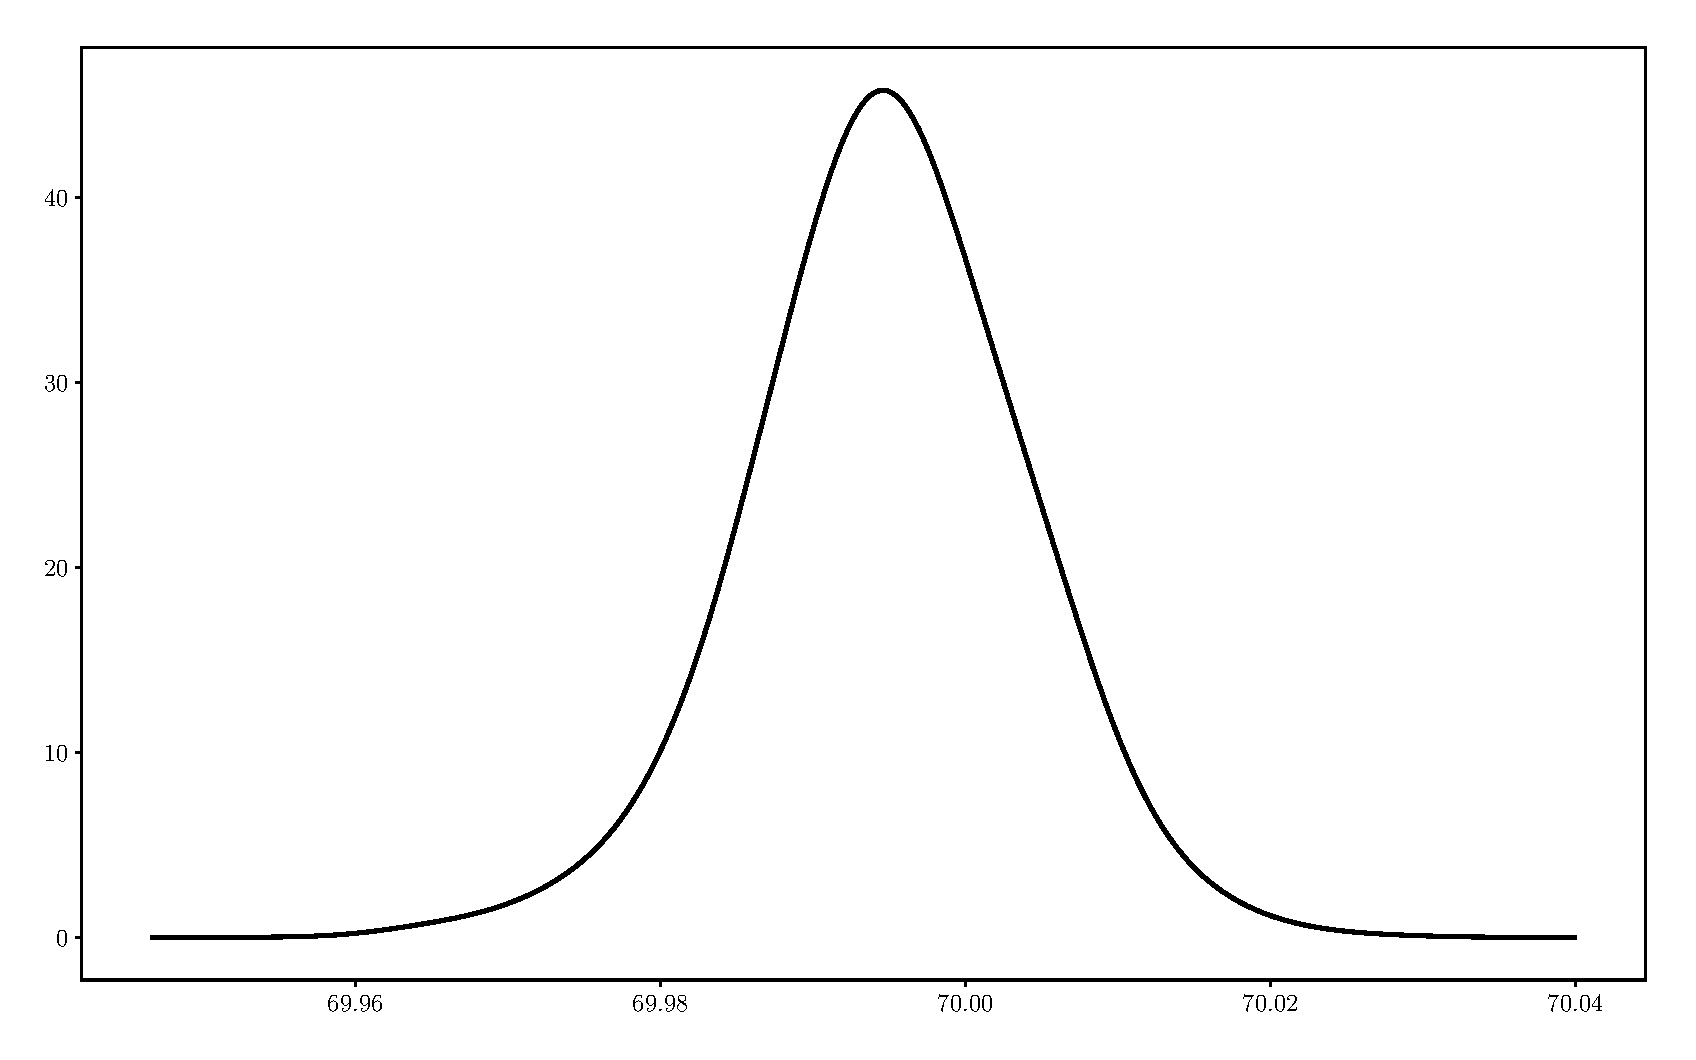
\includegraphics[width=\linewidth,keepaspectratio]{./figs/Case00/Model1_k1.eps}
\caption{Pdf of $k_1$}
\label{fig:s1a}
\end{subfigure}
\begin{subfigure}{.49\textwidth}
  \centering
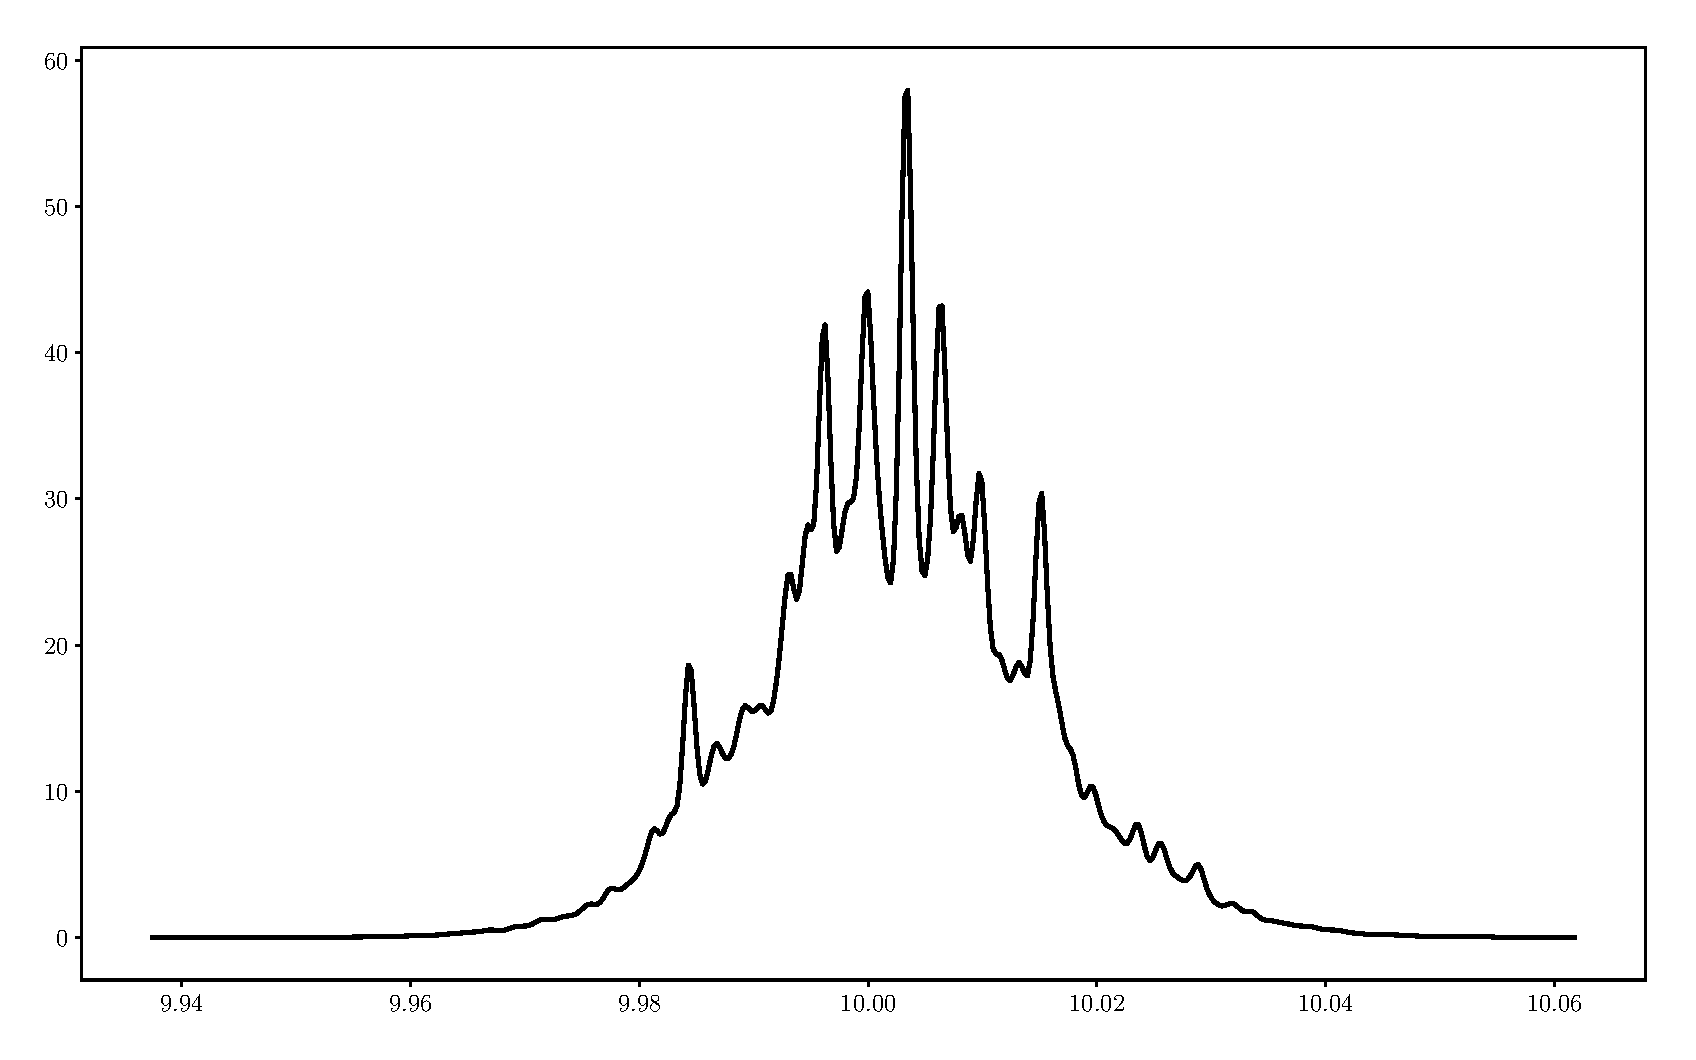
\includegraphics[width=\linewidth,keepaspectratio]{./figs/Case00/Model1_k2.eps}
\caption{Pdf of $k_2$}
\label{fig:s1b}
\end{subfigure}\\
\begin{subfigure}{.49\textwidth}
  \centering
\includegraphics[width=\linewidth,keepaspectratio]{./figs/Case00/Model1_c.eps}
\caption{Pdf of $c$}
\label{fig:s1c}
\end{subfigure}
\begin{subfigure}{.49\textwidth}
  \centering
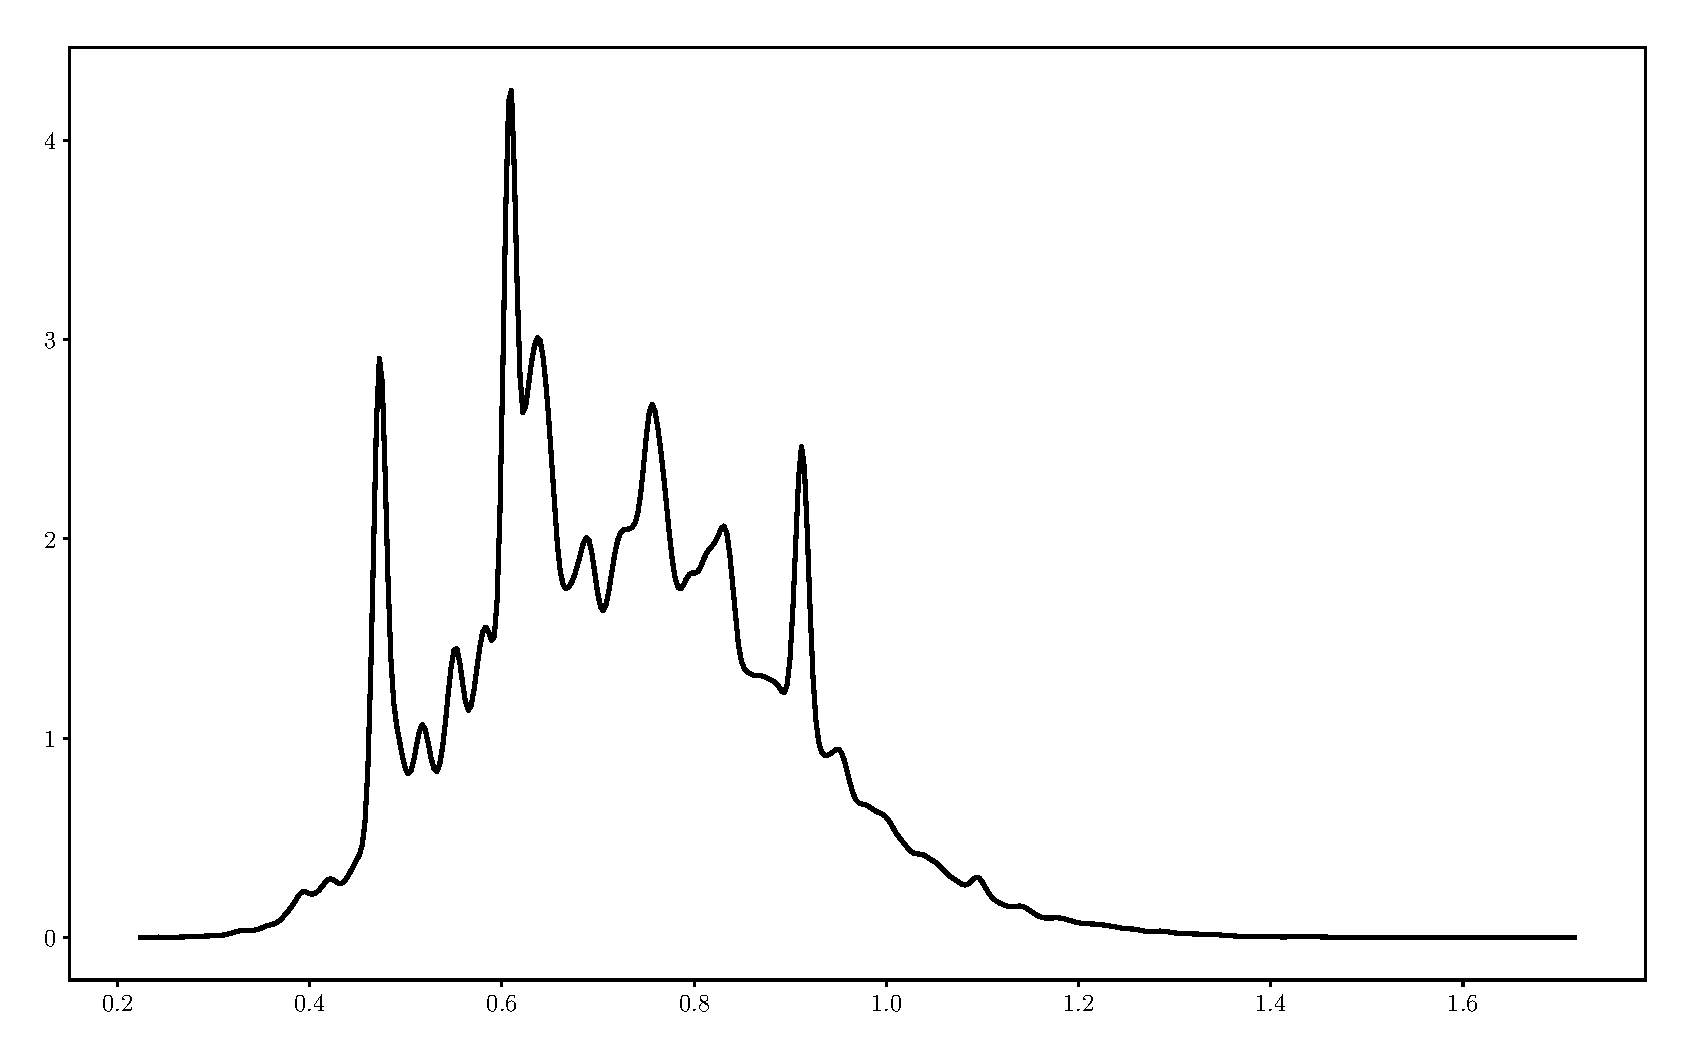
\includegraphics[width=\linewidth,keepaspectratio]{./figs/Case00/Model1_sigma.eps}
\caption{Pdf of $sigma$}
\label{fig:s1d}
\end{subfigure}\\
\begin{subfigure}{.49\textwidth}
  \centering
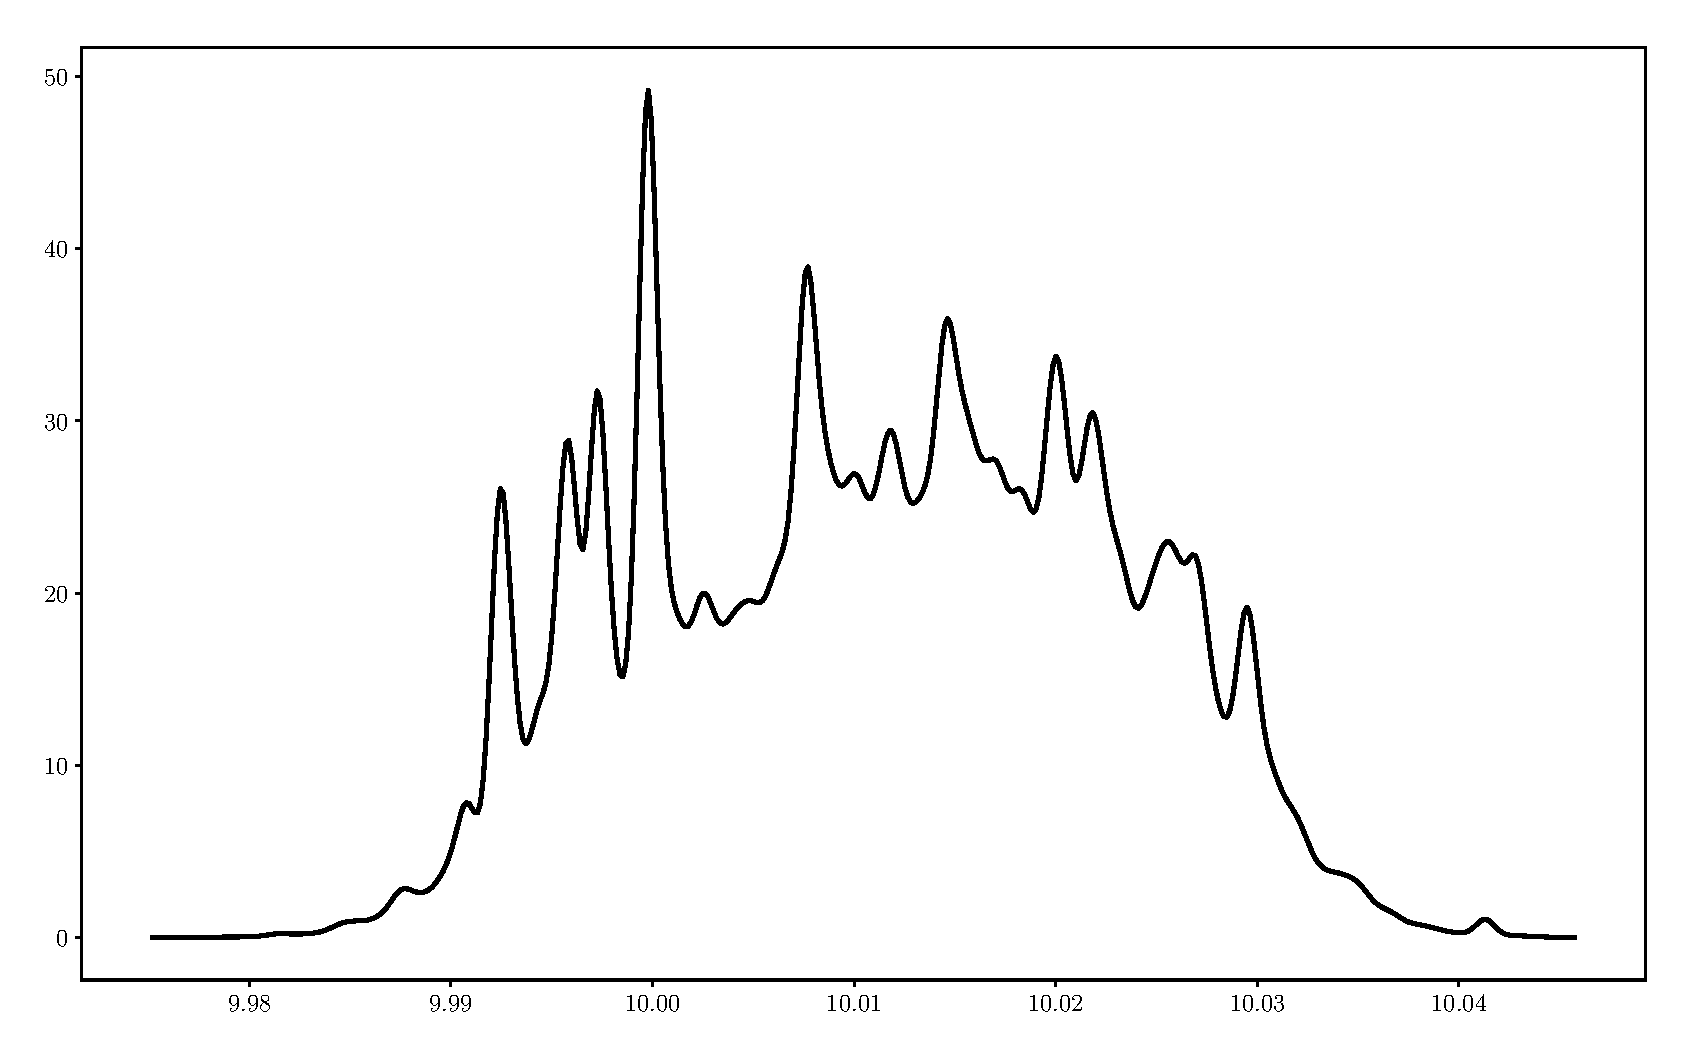
\includegraphics[width=\linewidth,keepaspectratio]{./figs/Case00/Model1_tsnaps.eps}
\caption{Pdf of $t_s$}
\label{fig:s1d}
\end{subfigure}
\end{figure}


\section*{Model 2}

A simplified model is presented here. The parameters are static and the stiffness is assumed to be constant throughout.

\begin{equation}
X_{k+1} = 
\begin{bmatrix}
1.0 & \Delta t \\
- \Delta t \frac{K}{m} & 1 - \Delta t \frac{c}{m}
\end{bmatrix}
+
%\begin{bmatrix}
%0 \\
%A \Delta t \cos(\omega t)
%\end{bmatrix}
%+
\begin{bmatrix}
0 \\
\sqrt(\Delta t) W_k
\end{bmatrix}
\end{equation}



\begin{figure}[!htb]
\centering
\begin{subfigure}{.49\textwidth}
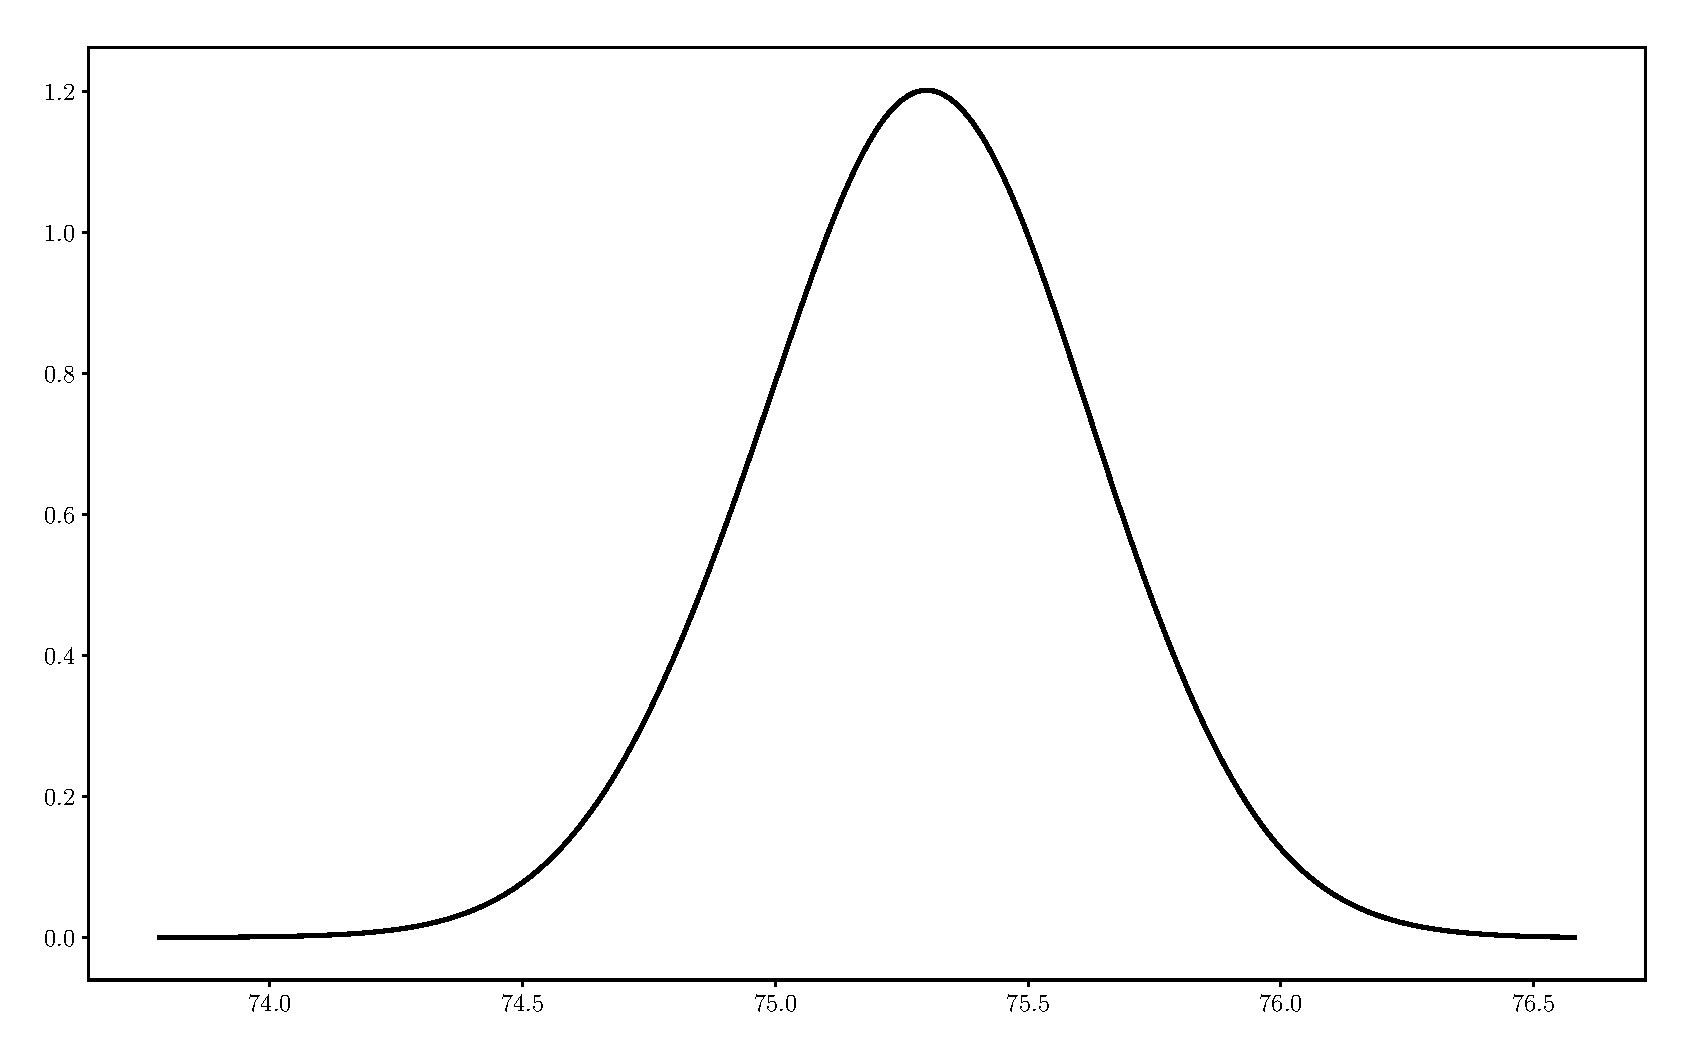
\includegraphics[width=\linewidth,keepaspectratio]{./figs/Case00/Model2_k.eps}
\caption{Pdf of $K$}
\end{subfigure}
\begin{subfigure}{.49\textwidth}
\centering
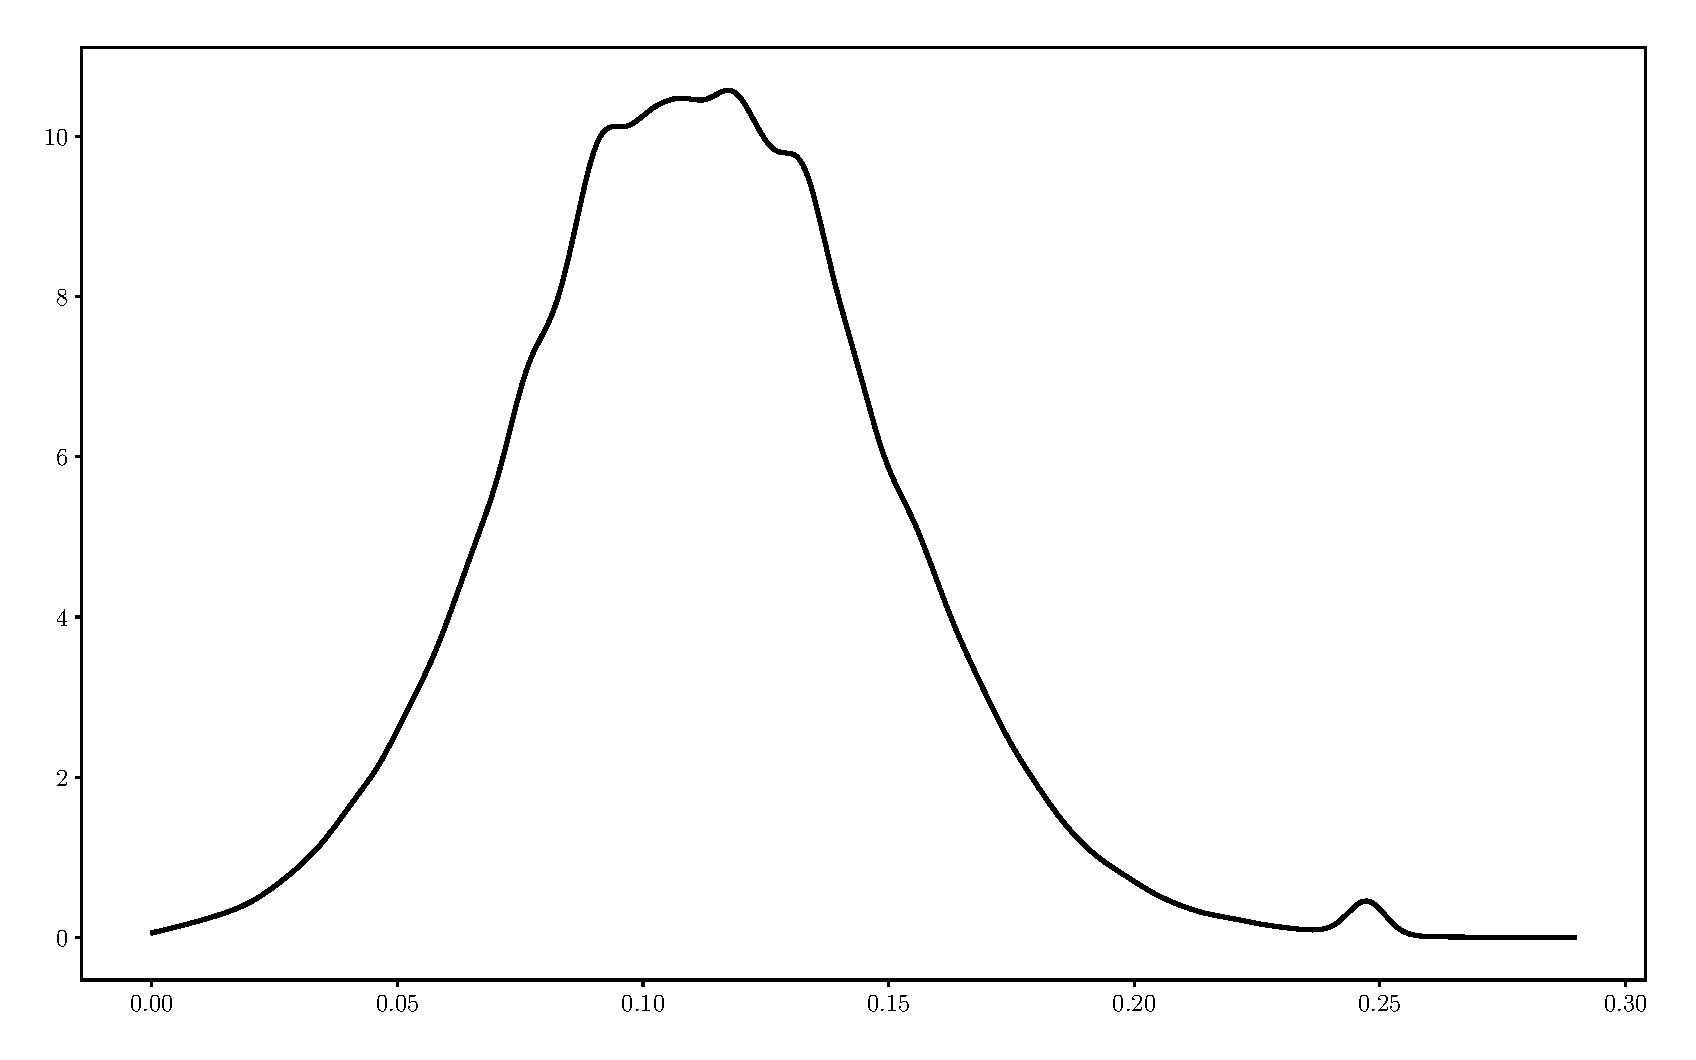
\includegraphics[width=\linewidth,keepaspectratio]{./figs/Case00/Model2_c.eps}
\caption{Pdf of $c$}
\label{fig:s1c}
\end{subfigure}\\
\begin{subfigure}{.49\textwidth}
\centering
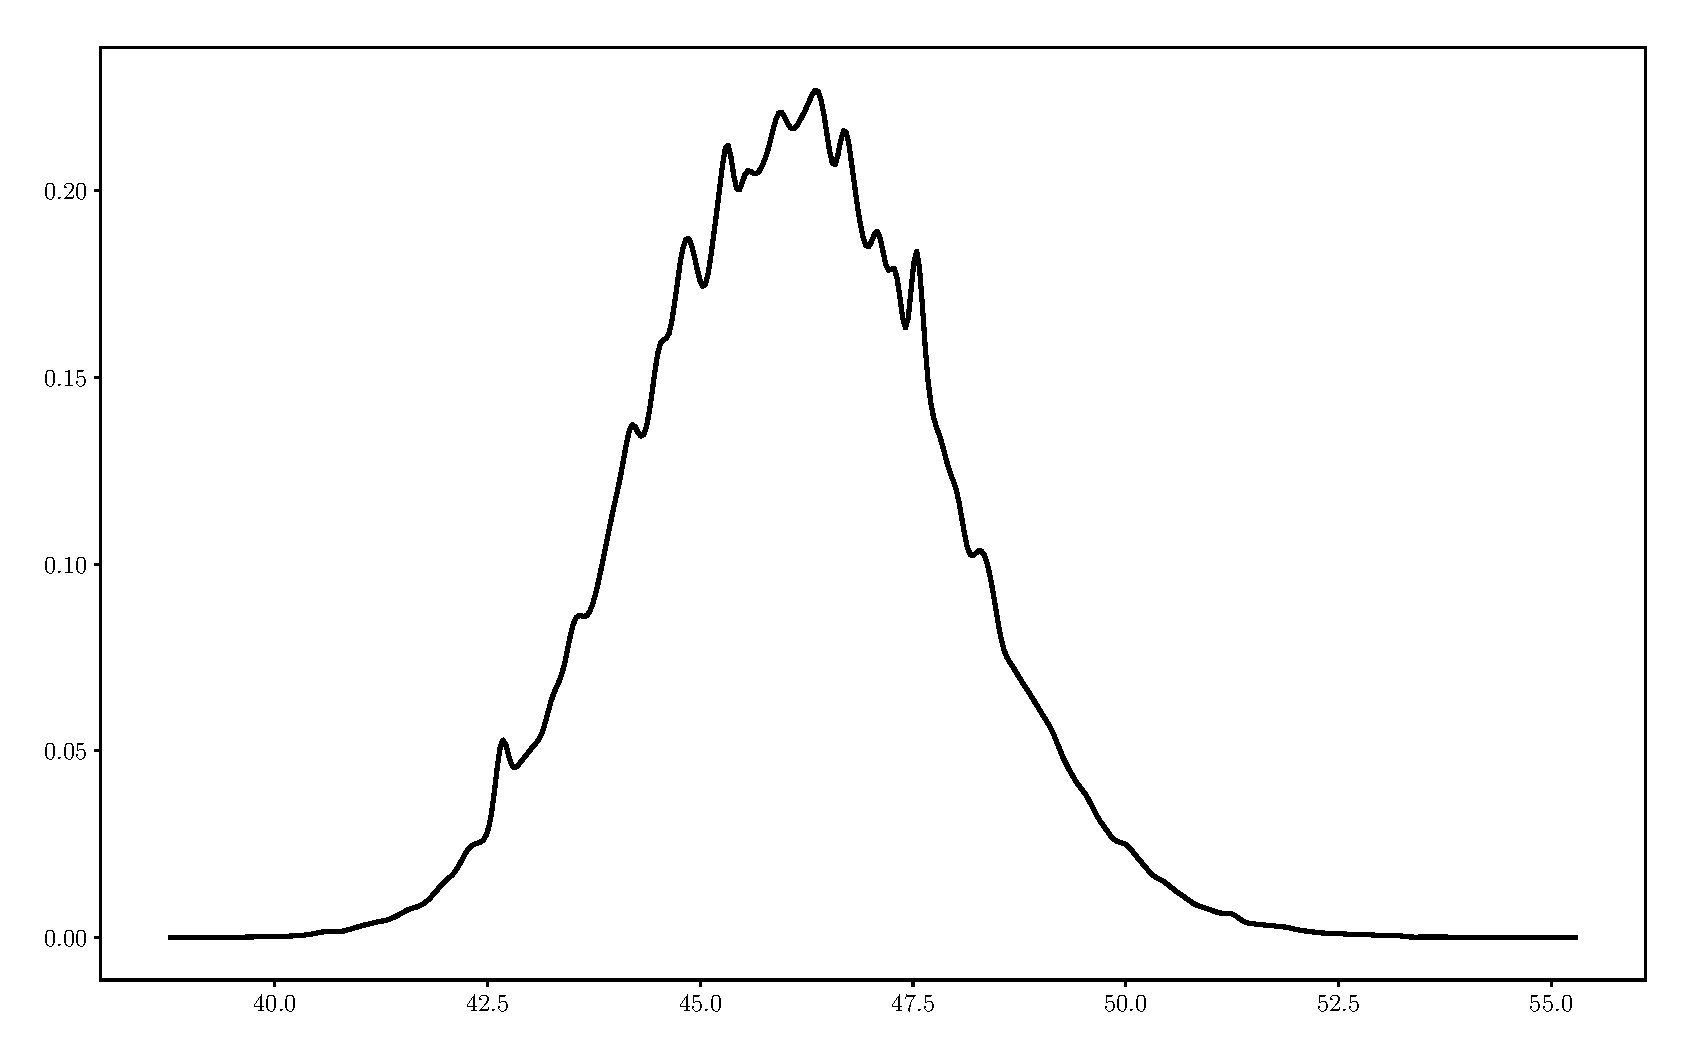
\includegraphics[width=\linewidth,keepaspectratio]{./figs/Case00/Model2_sigma.eps}
\caption{Pdf of $sigma$}
\label{fig:s1d}
\end{subfigure}
\end{figure}

\section*{Model 3}

The stiffness is described by a single parameter that is allowed to change. The damping and noise strength are static.
\begin{equation}
X_{k+1} = 
\begin{bmatrix}
1.0 & \Delta t & 0 \\
- \Delta t \frac{K}{m} & 1 - \Delta t \frac{c}{m} & 0 \\
0 & 0 & 1 
\end{bmatrix}
+
%\begin{bmatrix}
%0 \\
%A \Delta t \cos(\omega t)
%\end{bmatrix}
%+
\begin{bmatrix}
0 \\
\sqrt(\Delta t) \sigma W_k \\
\sqrt(\Delta t) \gamma Q_k
\end{bmatrix}
\end{equation}
where $Q_k$ is an independent GRV and $X = [x_1 x_2 x_3]$ where $x_1 = u$, $x_2 = \dot{u}$ and $x_3 = K$.


\begin{figure}[!htb]
\centering
\begin{subfigure}{.49\textwidth}
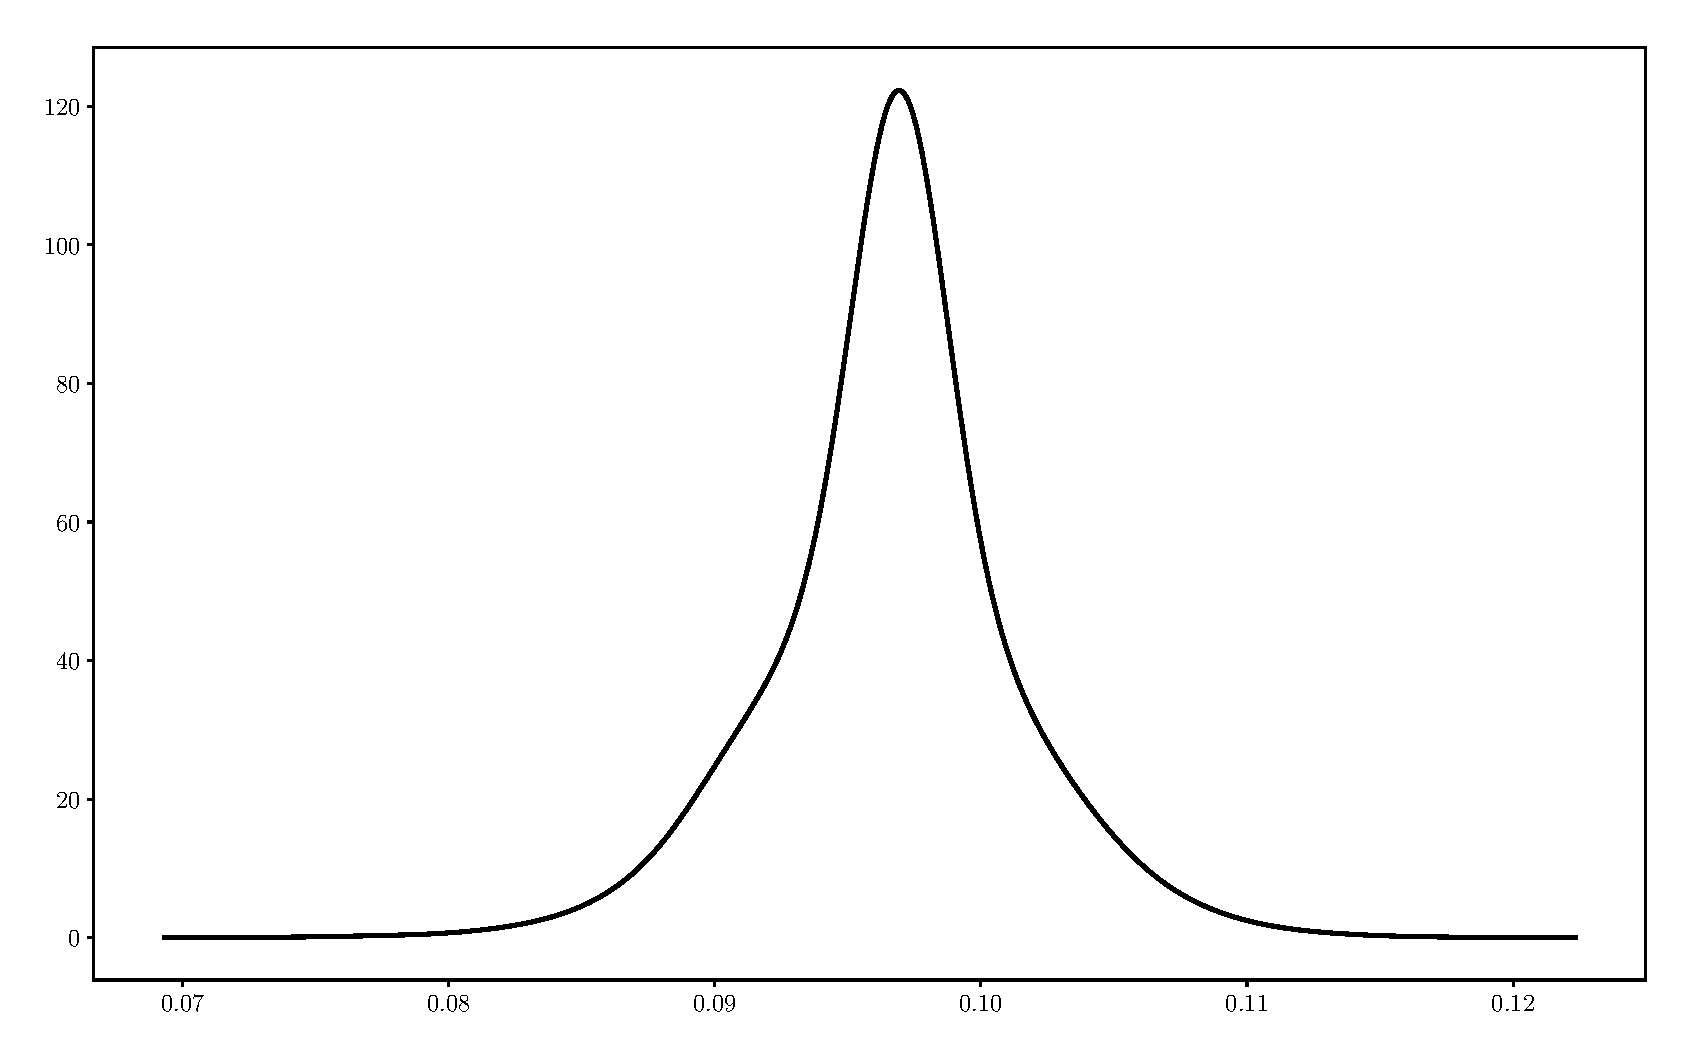
\includegraphics[width=\linewidth,keepaspectratio]{./figs/Case00/Model3_c.eps}
\caption{Pdf of $c$}
\end{subfigure}
\begin{subfigure}{.49\textwidth}
\centering
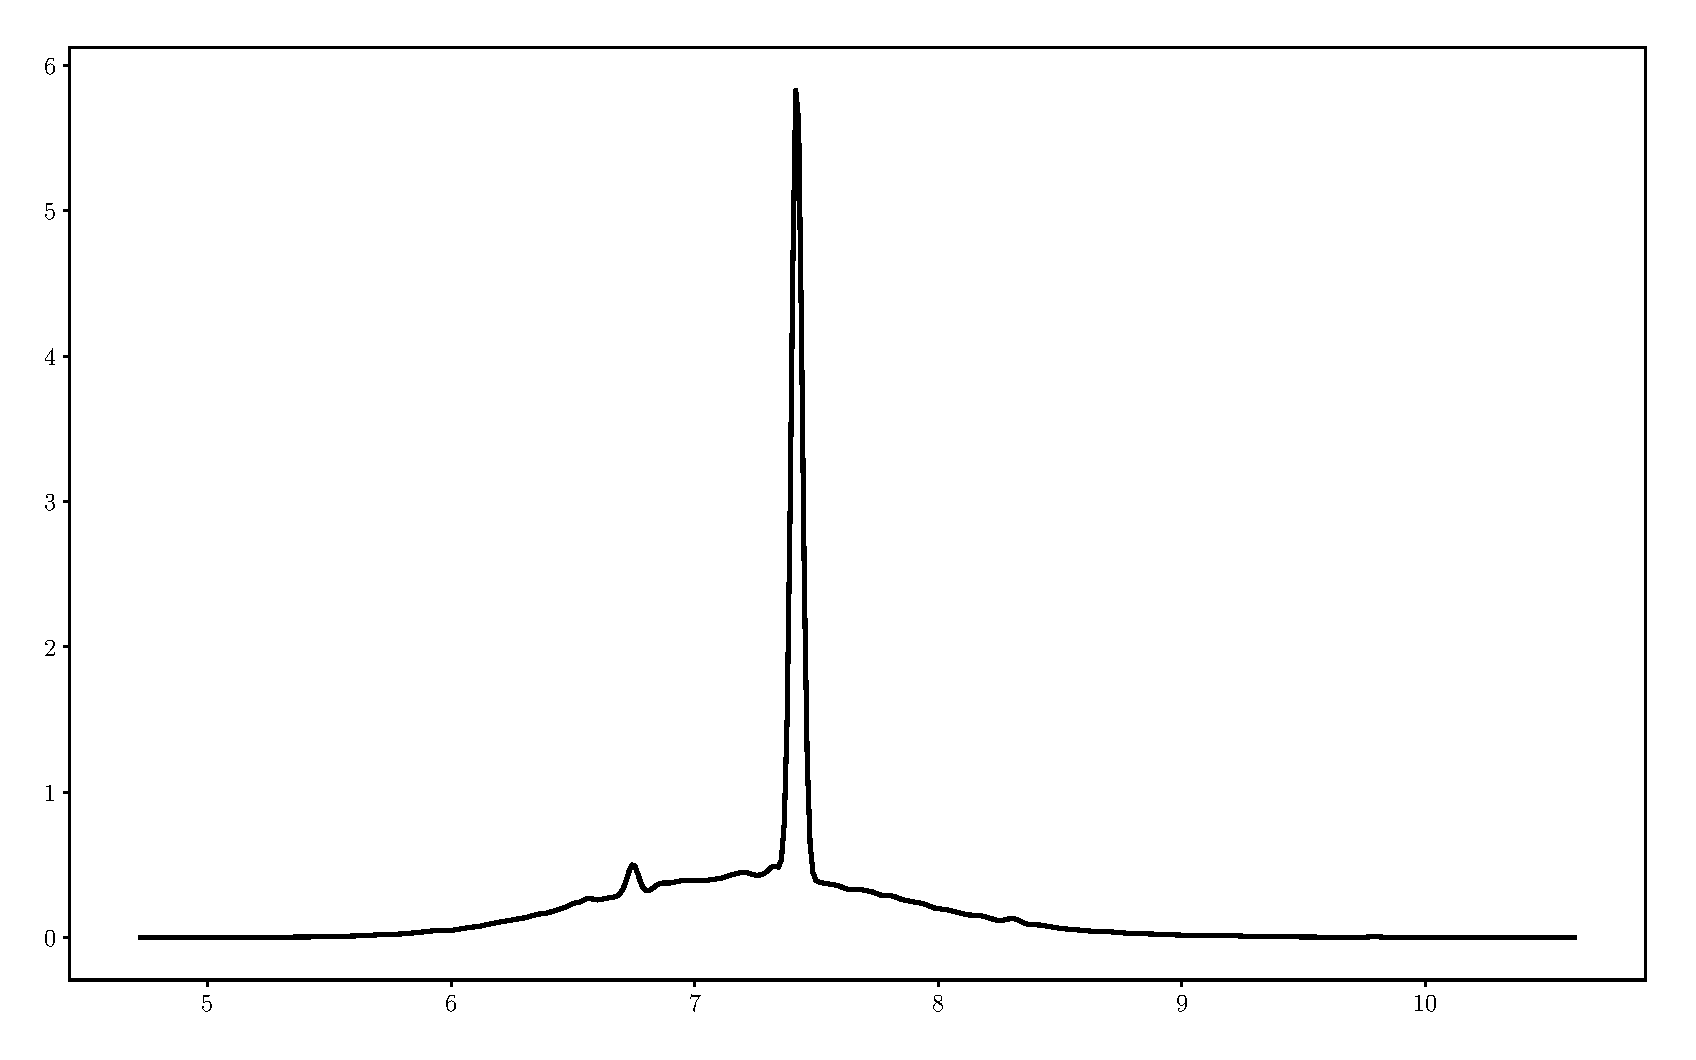
\includegraphics[width=\linewidth,keepaspectratio]{./figs/Case00/Model3_sigma.eps}
\caption{Pdf of $\sigma$}
\label{fig:s1c}
\end{subfigure}\\
\begin{subfigure}{.99\textwidth}
\centering
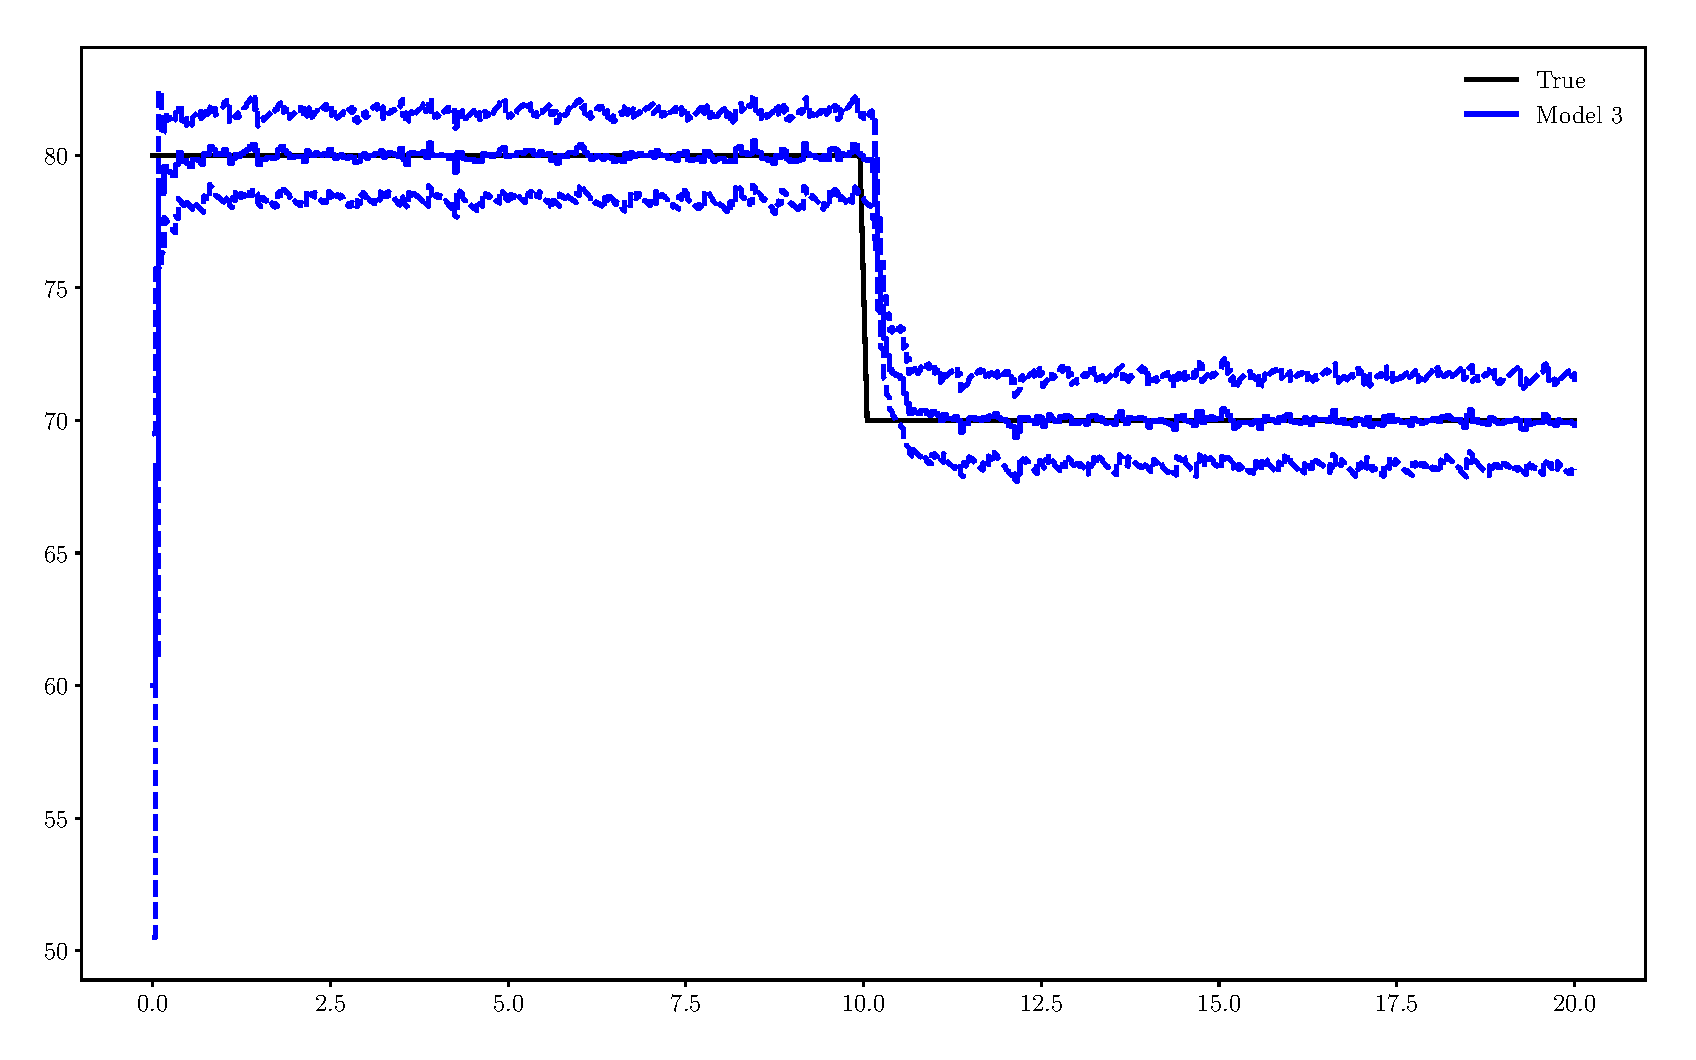
\includegraphics[width=\linewidth,keepaspectratio]{./figs/Case00/Model3_k_estimate.eps}
\caption{Mean and 99\% HPDI of $K$ using MAP estimates}
\label{fig:s1d}
\end{subfigure}
\end{figure}

\begin{figure}[!htb]
\centering
\begin{subfigure}{.49\textwidth}
\includegraphics[width=\linewidth,keepaspectratio]{./figs/Case00/Model3_BADIC_c.eps}
\caption{Pdf of $c$}
\end{subfigure}
\begin{subfigure}{.49\textwidth}
\centering
\includegraphics[width=\linewidth,keepaspectratio]{./figs/Case00/Model3_BADIC_sigma.eps}
\caption{Pdf of $\sigma$}
\label{fig:s1c}
\end{subfigure}\\
\begin{subfigure}{.99\textwidth}
\centering
\includegraphics[width=\linewidth,keepaspectratio]{./figs/Case00/Model3_BADIC_k_estimate.eps}
\caption{Mean and 99\% HPDI of $K$ using MAP estimates}
\label{fig:s1d}
\end{subfigure}
\end{figure}




\section*{Model 4}

The stiffness is described by a single parameter that is allowed to change. The damping and noise strength are static. The value of $\gamma$ is estimated. 

\begin{figure}[!htb]
\centering
\begin{subfigure}{.49\textwidth}
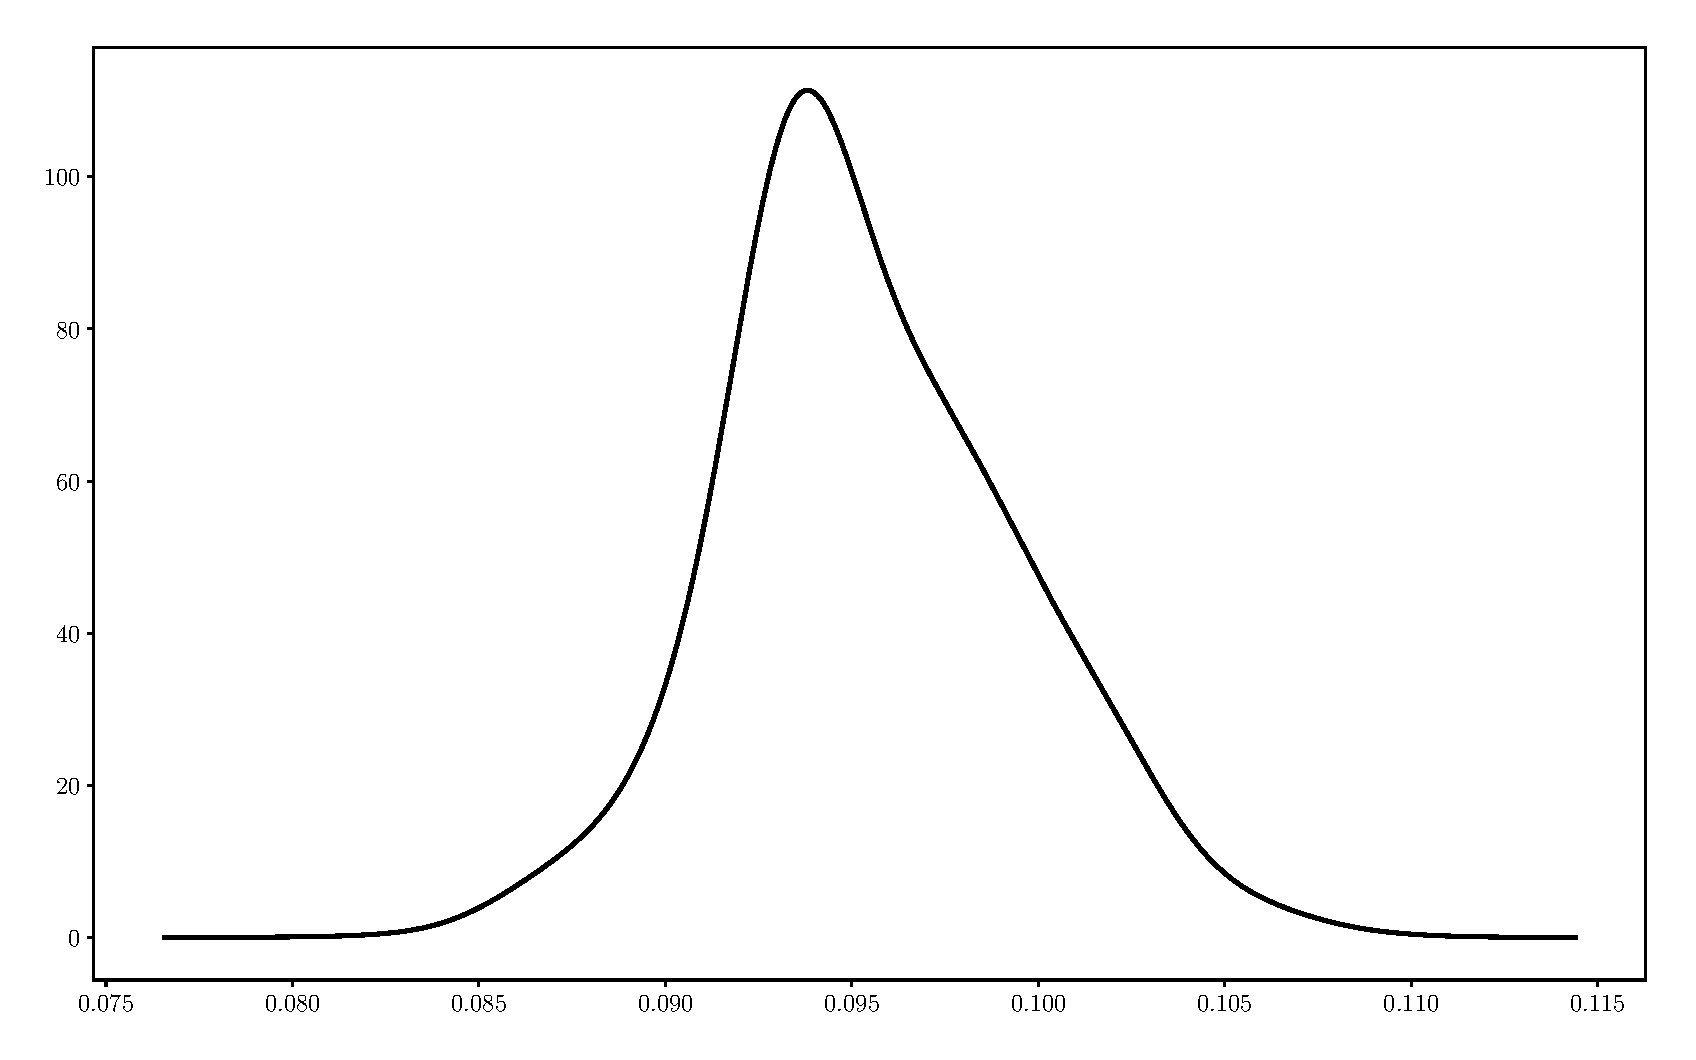
\includegraphics[width=\linewidth,keepaspectratio]{./figs/Case00/Model4_c.eps}
\caption{Pdf of $c$}
\end{subfigure}
\begin{subfigure}{.49\textwidth}
\centering
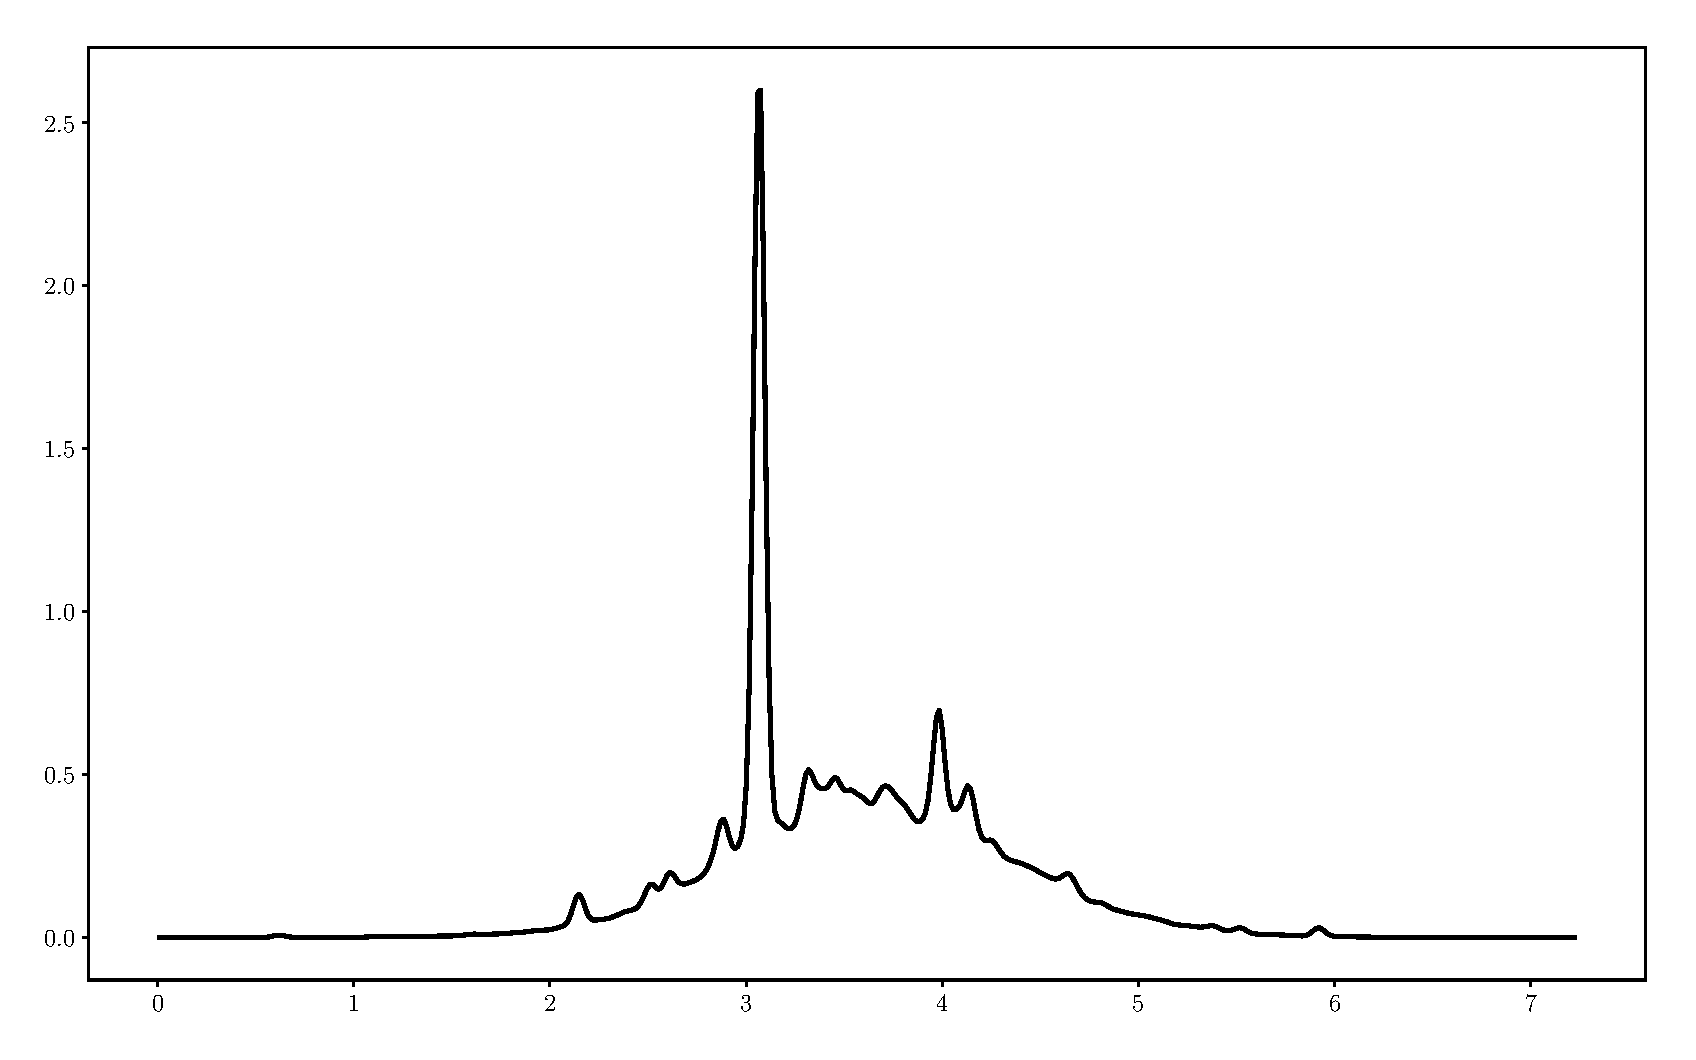
\includegraphics[width=\linewidth,keepaspectratio]{./figs/Case00/Model4_sigma.eps}
\caption{Pdf of $\sigma$}
\label{fig:s1c}
\end{subfigure}\\
\begin{subfigure}{.49\textwidth}
\centering
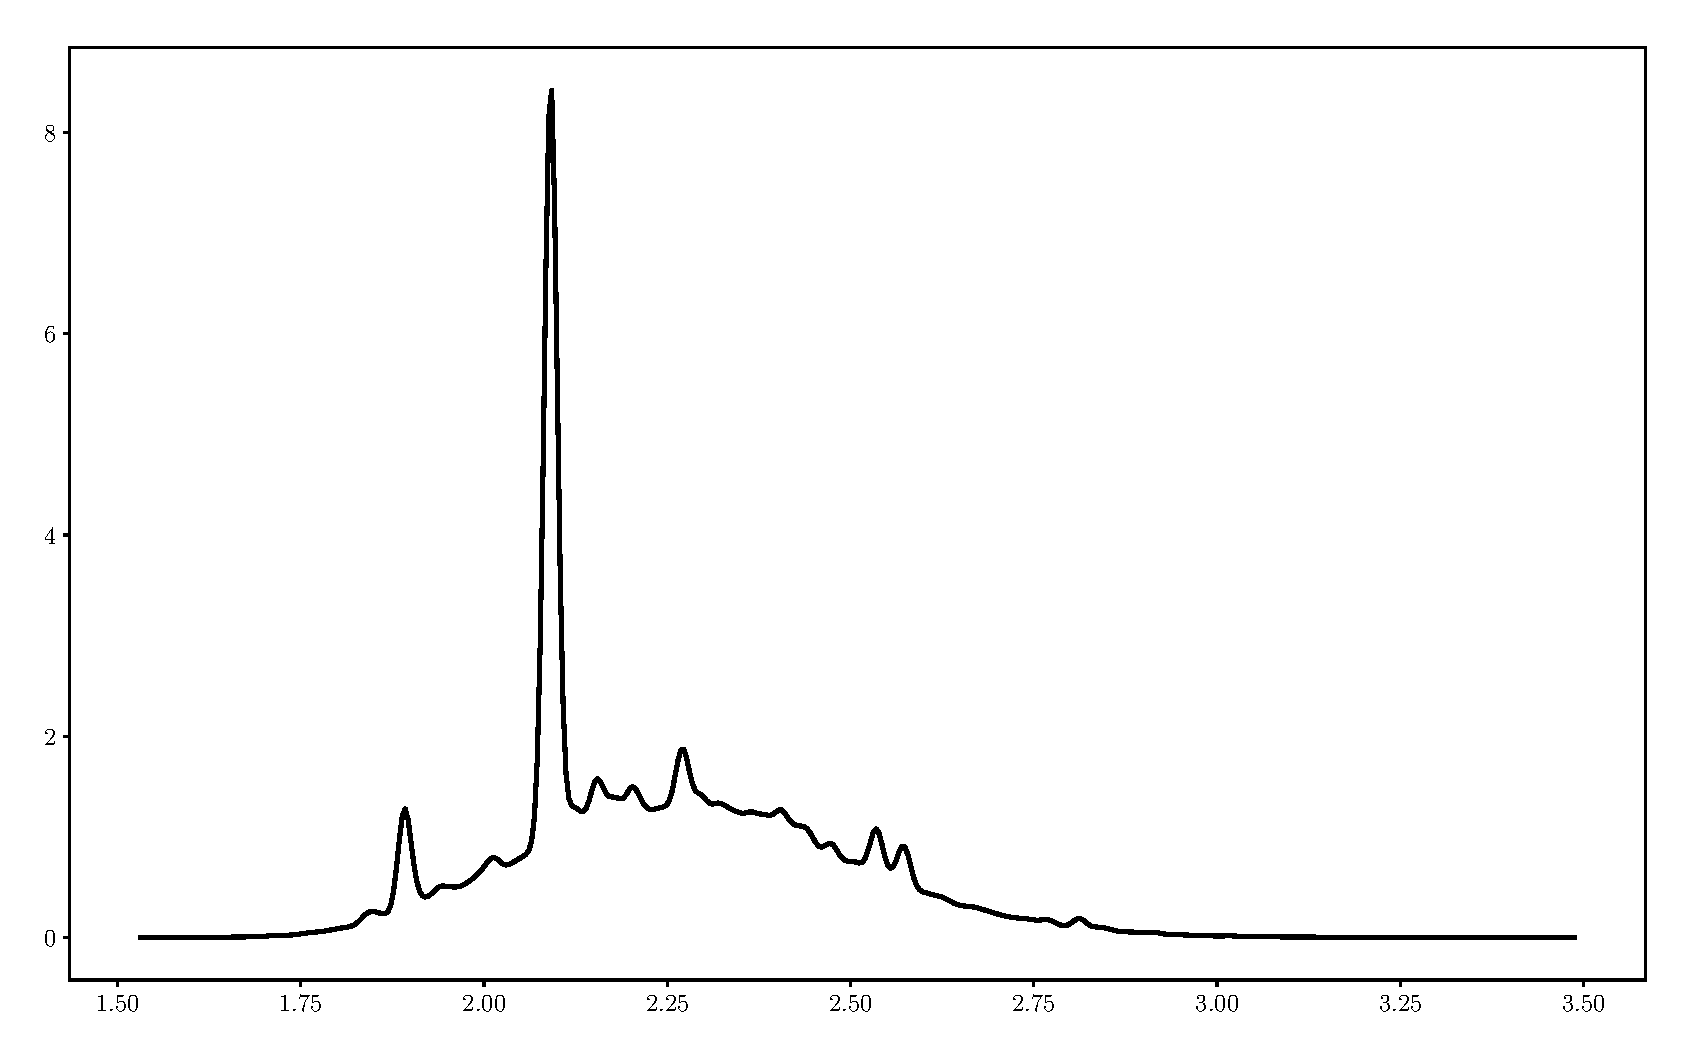
\includegraphics[width=\linewidth,keepaspectratio]{./figs/Case00/Model4_gamma.eps}
\caption{Pdf of $\gamma$}
\label{fig:s1c}
\end{subfigure}\\
\begin{subfigure}{.99\textwidth}
\centering
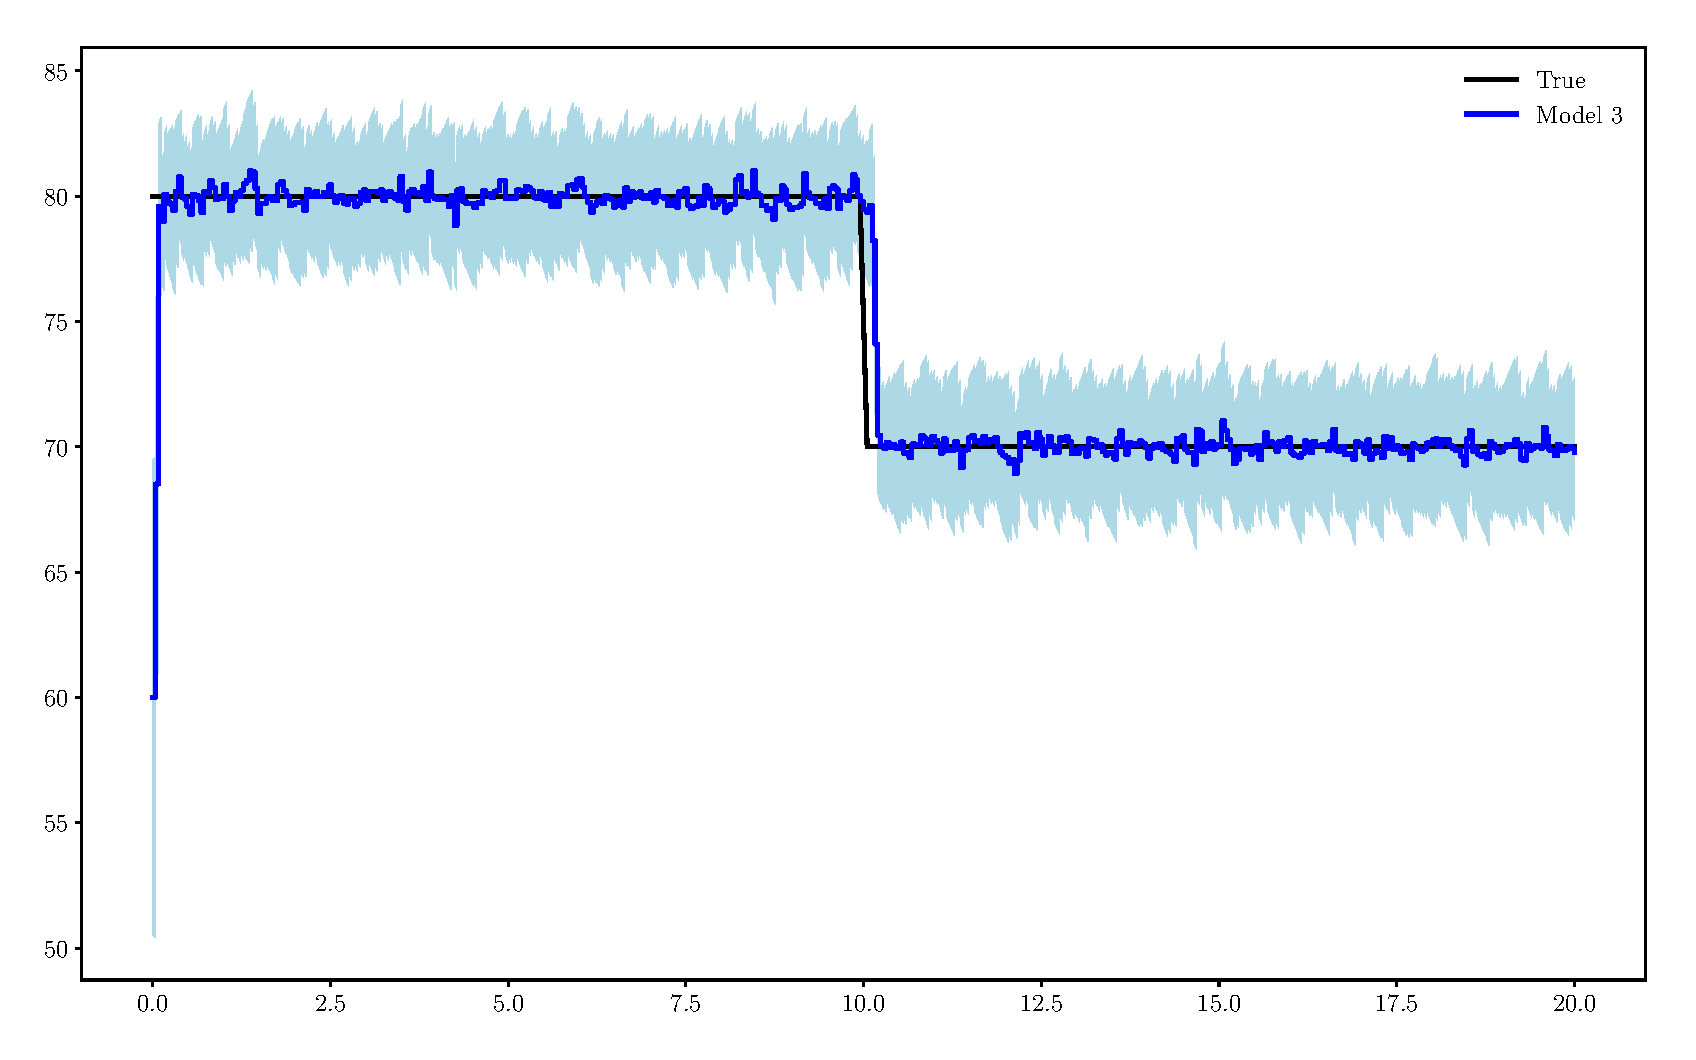
\includegraphics[width=\linewidth,keepaspectratio]{./figs/Case00/Model4_k_estimate.eps}
\caption{Mean and 99\% HPDI of $K$ using MAP estimates}
\label{fig:s1d}
\end{subfigure}
\end{figure}

\begin{figure}[!htb]
\centering
\begin{subfigure}{.49\textwidth}
\includegraphics[width=\linewidth,keepaspectratio]{./figs/Case00/Model4_BADIC_c.eps}
\caption{Pdf of $c$}
\end{subfigure}
\begin{subfigure}{.49\textwidth}
\centering
\includegraphics[width=\linewidth,keepaspectratio]{./figs/Case00/Model4_BADIC_sigma.eps}
\caption{Pdf of $\sigma$}
\label{fig:s1c}
\end{subfigure}\\
\begin{subfigure}{.49\textwidth}
\centering
\includegraphics[width=\linewidth,keepaspectratio]{./figs/Case00/Model4_BADIC_gamma.eps}
\caption{Pdf of $\gamma$}
\label{fig:s1c}
\end{subfigure}\\
\begin{subfigure}{.99\textwidth}
\centering
\includegraphics[width=\linewidth,keepaspectratio]{./figs/Case00/Model4_BADIC_k_estimate.eps}
\caption{Mean and 99\% HPDI of $K$ using MAP estimates}
\label{fig:s1d}
\end{subfigure}
\end{figure}


\section*{Model 5}

The stiffness is described by a single parameter that is allowed to change. The damping and noise strength are static. The value of $\gamma$ is estimated. 

\begin{figure}[!htb]
\centering
\begin{subfigure}{.49\textwidth}
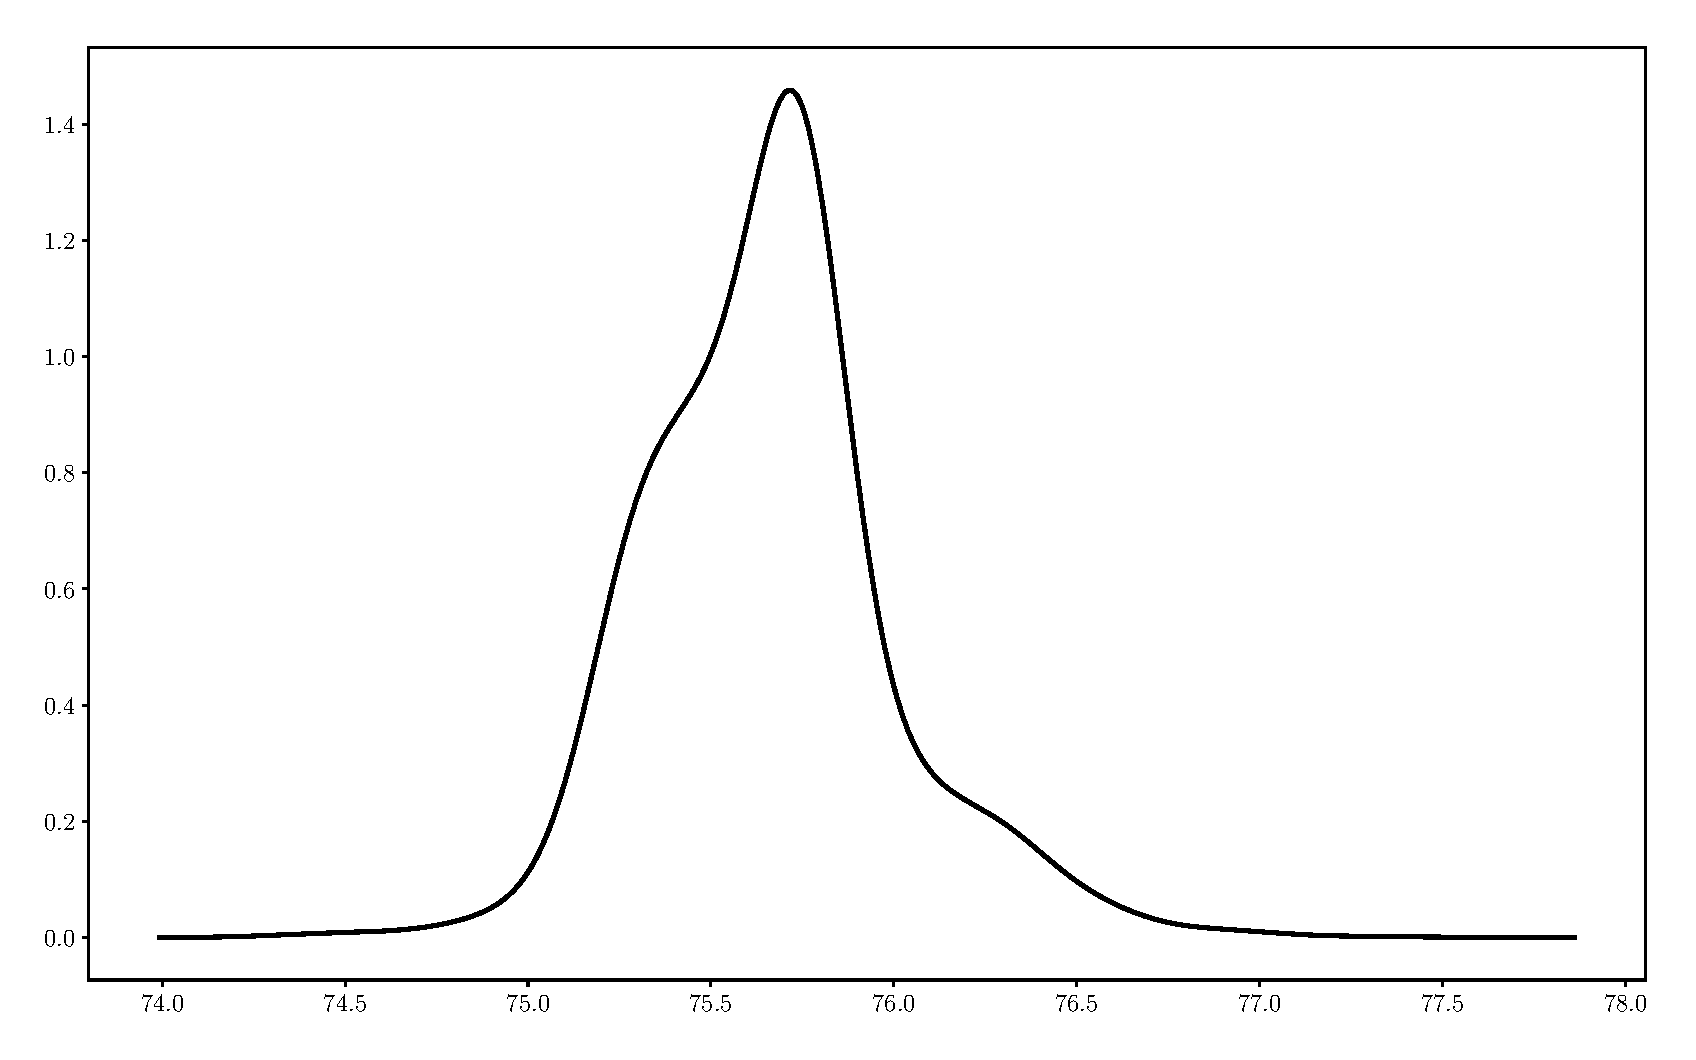
\includegraphics[width=\linewidth,keepaspectratio]{./figs/Case00/Model5_k.eps}
\caption{Pdf of $K$}
\end{subfigure}
\begin{subfigure}{.49\textwidth}
\centering
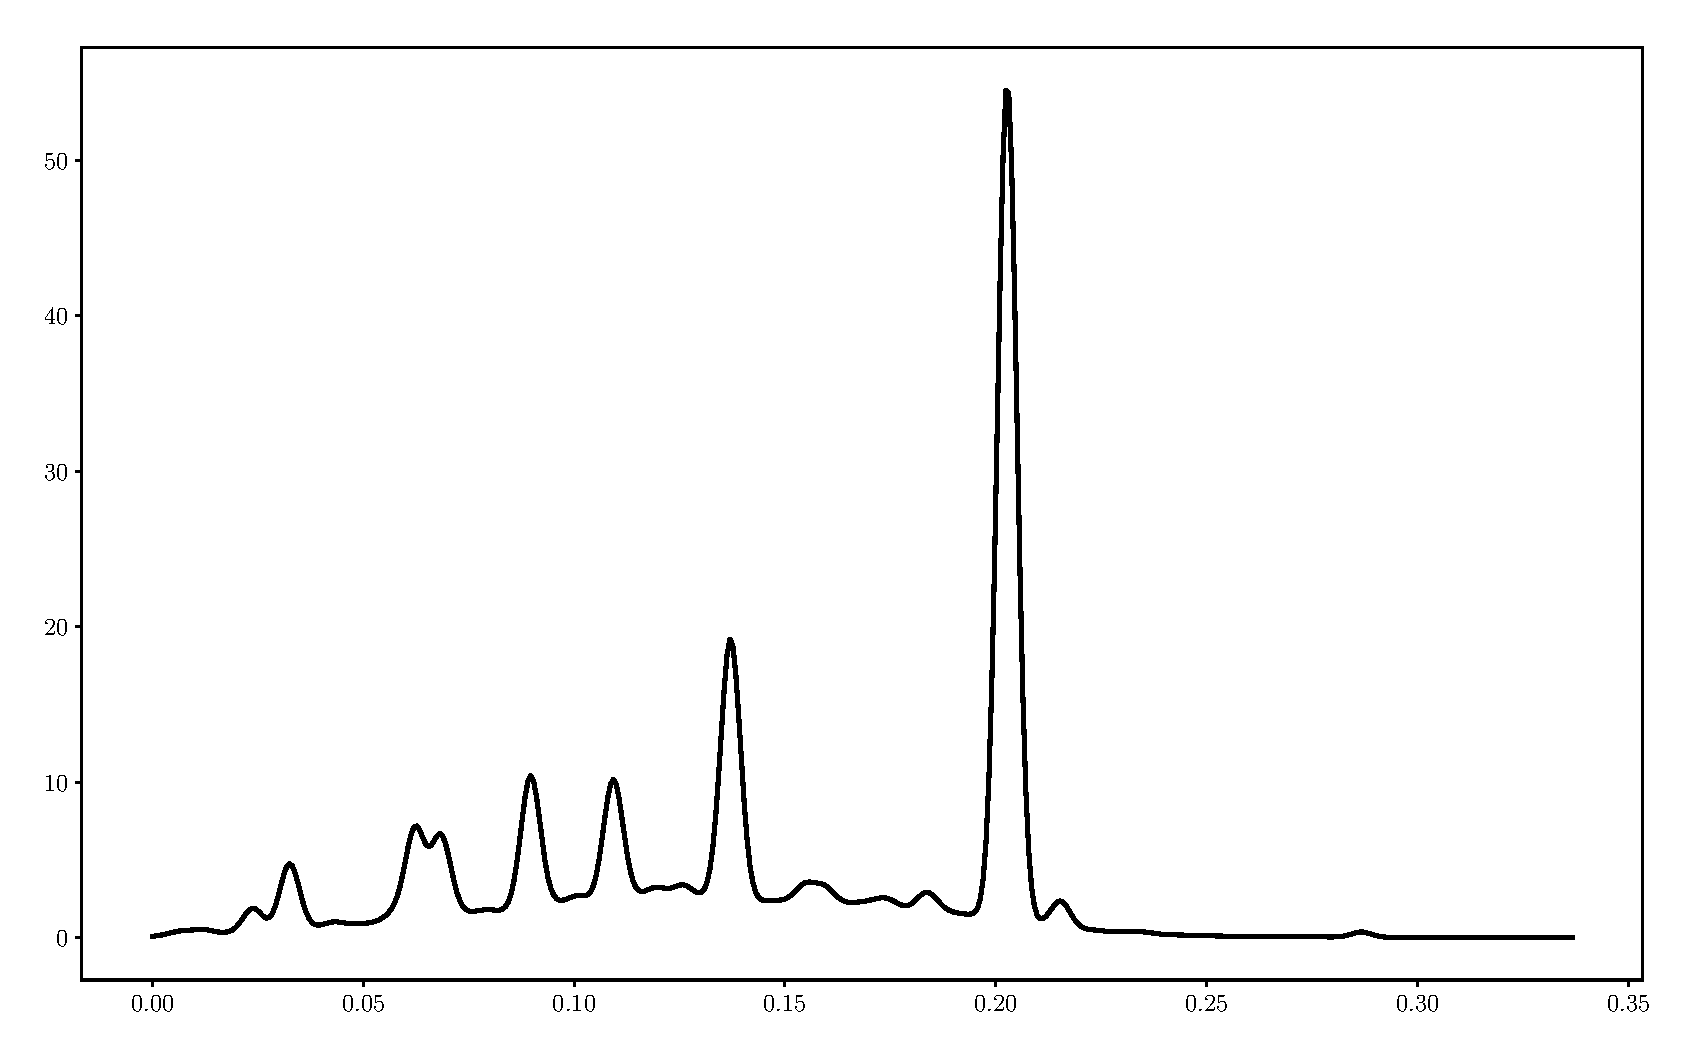
\includegraphics[width=\linewidth,keepaspectratio]{./figs/Case00/Model5_c.eps}
\caption{Pdf of $c$}
\label{fig:s1c}
\end{subfigure}\\
\begin{subfigure}{.49\textwidth}
\centering
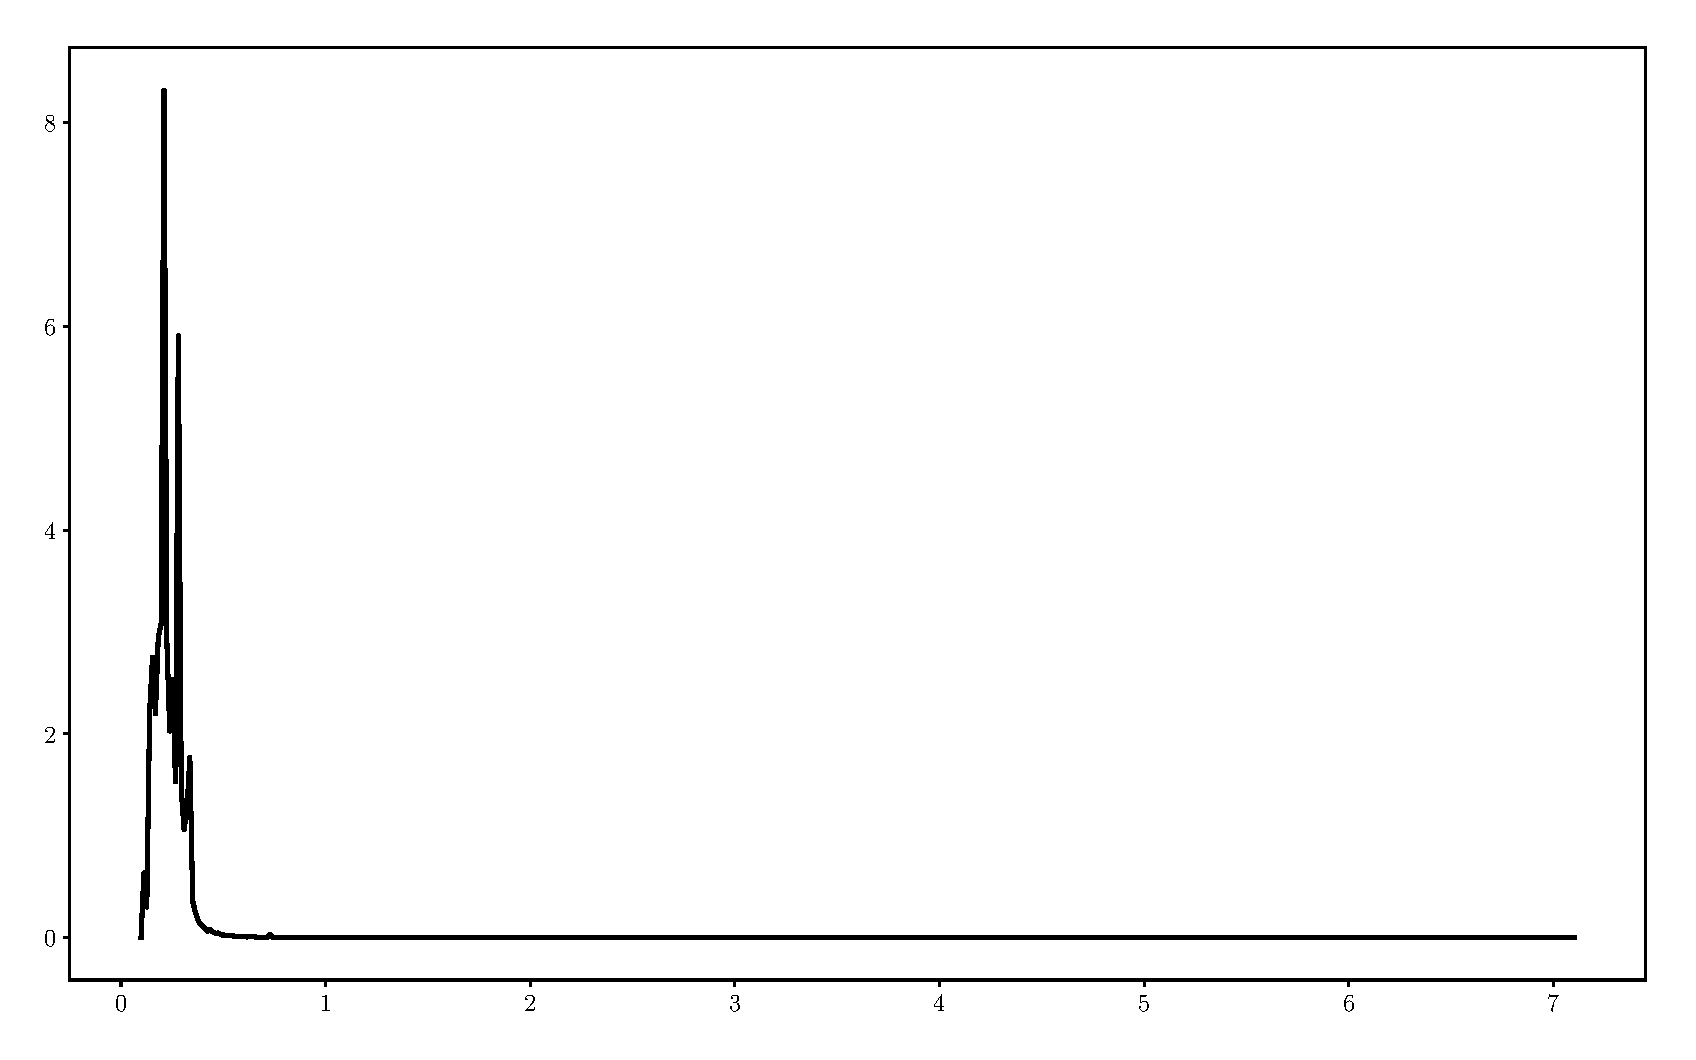
\includegraphics[width=\linewidth,keepaspectratio]{./figs/Case00/Model5_tau.eps}
\caption{Pdf of $\tau$}
\label{fig:s1c}
\end{subfigure}
\begin{subfigure}{.49\textwidth}
\centering
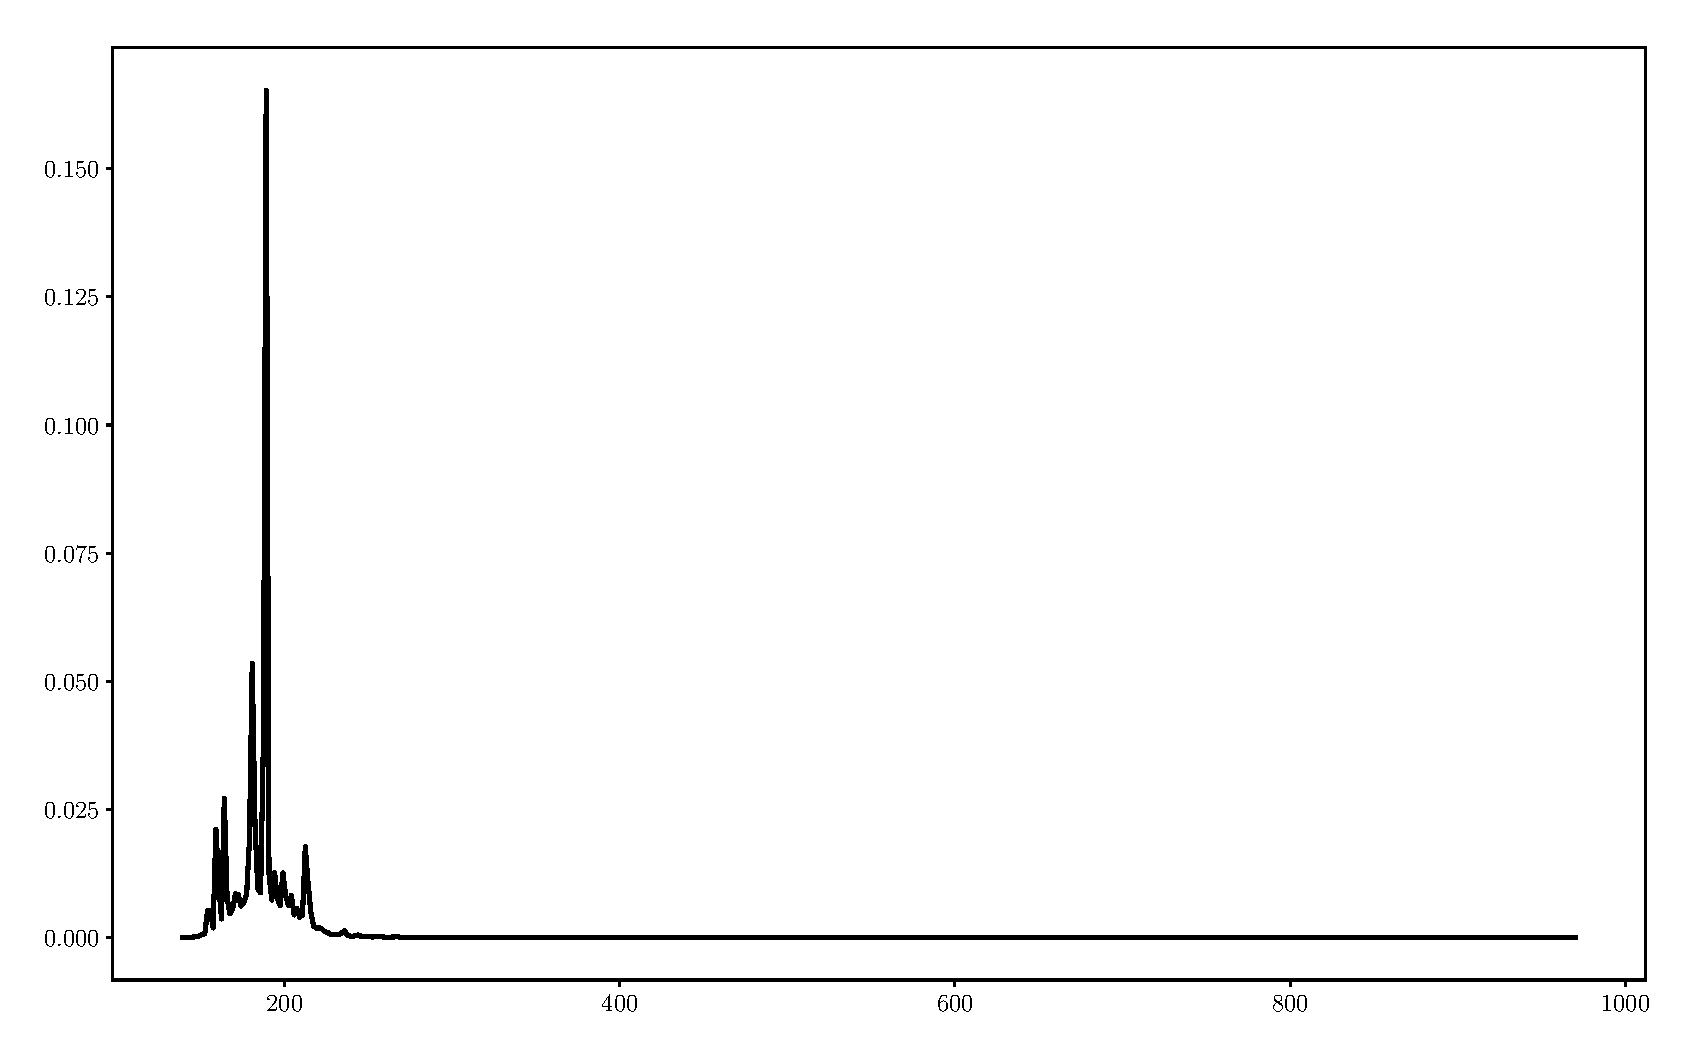
\includegraphics[width=\linewidth,keepaspectratio]{./figs/Case00/Model5_sigma.eps}
\caption{Pdf of $\sigma$}
\label{fig:s1c}
\end{subfigure}\\
\end{figure}

\section*{Model 6}

\begin{figure}[!htb]
\centering
\begin{subfigure}{.49\textwidth}
\includegraphics[width=\linewidth,keepaspectratio]{./figs/Case00/Model6_c.eps}
\caption{Pdf of $c$}
\end{subfigure}
\begin{subfigure}{.49\textwidth}
\centering
\includegraphics[width=\linewidth,keepaspectratio]{./figs/Case00/Model6_sigma.eps}
\caption{Pdf of $\sigma$}
\label{fig:s1c}
\end{subfigure}\\
\begin{subfigure}{.49\textwidth}
\centering
\includegraphics[width=\linewidth,keepaspectratio]{./figs/Case00/Model6_gamma.eps}
\caption{Pdf of $\gamma$}
\label{fig:s1c}
\end{subfigure}
\begin{subfigure}{.49\textwidth}
\centering
\includegraphics[width=\linewidth,keepaspectratio]{./figs/Case00/Model6_k0.eps}
\caption{Pdf of $E[K(0)$}
\label{fig:s1c}
\end{subfigure}\\
\begin{subfigure}{.99\textwidth}
\centering
\includegraphics[width=\linewidth,keepaspectratio]{./figs/Case00/Model6_k_estimate.eps}
\caption{Mean and 99\% HPDI of $K$ using MAP estimates}
\label{fig:s1d}
\end{subfigure}
\end{figure}


\subsection{Model selection results}


The priors of static parameters estimated using MCMC are shown in Table~\ref{table:case00:priors}. $U[a,b]$ denotes a uniform distribution between $a$ and $b$. A scalar value denotes that the value is fixed and assumed known for this simulation, it is not estimated for that model. An empty cell signifies that this parameter is not present in the model.

\begin{table}[!h]
\caption{Prior parameter distributions.}
\resizebox{\linewidth}{!}{%
\centering
\begin{tabular}{l|ccccccccc}
\hline
					&	$k_1$		&	$k_2$		&	$K$			&	$c$			&	$t_s$		&	$\sigma$	&	$\gamma$	&	$\tau$		&	$E[K(0)]$	\\
\hline																			
$\mathcal{M}_1$		&	$U[0,1000]$	&	$U[0,1000]$	&				&	$U[0,5]$	&	$U[0,20]$	&	$U[0,1000]$	&				&				&		\\
$\mathcal{M}_2$		&				&				&	$U[0,1000]$	&	$U[0,5]$	&				&	$U[0,1000]$	&				&				&		\\
$\mathcal{M}_3$		&				&				&				&	$U[0,5]$	&				&	$U[0,1000]$	&	1			&				&	60	\\
$\mathcal{M}_3^*$	&				&				&				&	$U[0,5]$	&				&	$U[0,1000]$	&	1			&				&	5	\\
$\mathcal{M}_4$		&				&				&				&	$U[0,5]$	&				&	$U[0,1000]$	&	$U[0,1000]$	&				&	60	\\
$\mathcal{M}_4^*$	&				&				&				&	$U[0,5]$	&				&	$U[0,1000]$	&	$U[0,1000]$	&				&	5	\\
$\mathcal{M}_5$		&				&				&	$U[0,1000]$	&	$U[0,5]$	&				&	$U[0,1000]$	&				&	$U[0,10]$	&		\\
$\mathcal{M}_6$		&				&				&				&	$U[0,5]$	&				&	$U[0,1000]$	&	$U[0,1000]$	&				&	$U[0,100]$	\\
\hline
\end{tabular}
}
\label{table:case00:priors}
\end{table}


\begin{table}[!htb]
\begin{tabular}{l|lll}
\hline
Name & Static parameters & Time-varying parameters & Known parameters   \\
\hline
$\mathcal{M}_1$ & $c$, $k_1$, $k_2$, $\sigma$, $t_s$ &  & $m$, $\vec{\mu}_0$, $\vec{P}_0$    \\
$\mathcal{M}_2$ & $c$, $K$, $\sigma$ &  & $m$, $\vec{\mu}_0$, $\vec{P}_0$   \\
$\mathcal{M}_3$ & $c$, $\sigma$ & $K$ & $m$, $\gamma$, $\vec{\mu}_0$, $\vec{P}_0$ \\
$\mathcal{M}_4$ & $c$, $\sigma$, $\gamma$ & $K$ & $m$, $\vec{\mu}_0$, $\vec{P}_0$  \\
$\mathcal{M}_5$ & $c$, $K$, $\sigma$, $\tau$ & & $m$, $\vec{\mu}_0$, $\vec{P}_0$ \\
$\mathcal{M}_6$ & $c$, $\sigma$, $E[K(0)]$, $\gamma$ & $K$ & $m$, $E[X(0)]$, $E[V(0)]$,  $\vec{P}_0$   \\
\hline
\end{tabular}
\end{table}

\begin{table}[!h]
\caption{Evidence of proposed models for the numerical nonlinear aeroelastic system.}
\centering
\resizebox{\linewidth}{!}{%
\begin{tabular}{l|cccccccccc}
\hline
Model & $\mathcal{M}_1$ & $\mathcal{M}_2$ & $\mathcal{M}_3$ & $\mathcal{M}_3^*$ &  $\mathcal{M}_4$ & $\mathcal{M}_4^*$ & $\mathcal{M}_5$ & $\mathcal{M}_6$ \\
\hline
log Evidence 								&	327.7	&	-212.2	&	80.6	&	-992.7	&	112.8	&	-327.0	&	-122.5	&	129.6	\\
Average data-fit 							&	370.5	&	-197.2	&	91.7	&	-987.0	&	131.5	&	-314.6	&	-105.4	&	150.4	\\
EIG											&	42.7	&	15.1	&	11.1	&	5.7		&	18.7	&	12.4	&	17.1	&	20.8	\\
\hline																					
Probability \% ($\vec{\mathcal{M}}_a$)		&	100.0		&	0.0		&	0.0		&	0.0		&	0.0		&	0.0	&	0.0		&	0.0		\\
\hline																					
\end{tabular}
}
\label{table:case00:evidence}
\end{table}

The full model is selected. Notice that the addition of colored noise to model $\mathcal{M}_2$ increases the evidence of that model. The models that perform best after the generating models, are the models that treat the stiffness as a time-varying parameter. Notice the impact of bad initial guess of the prior mean of the stiffness. The evidence significantly drops from models $\mathcal{M}_3$ and $\mathcal{M}_4$ to $\mathcal{M}_3^*$ and $\mathcal{M}_4^*$. The evidence is still higher for models $\mathcal{4}$ and $\mathcal{4}^*$ since the tuning parameter $\gamma$ is also estimated. When the initial mean of $K$ is estimated, the evidence is significantly higher. The evidence of models $\mathcal{3}^*$ and $\mathcal{M}_4^*$ shows the influence of bad initial conditions.


\section{Sensor}

Consider a similar MSD system where the spring doesn't snap but the sensor has a drift. Consider a sensor that, due to age, is not properly calibrated such that the true sensor dynamics are
\begin{equation}
d_k = u_k + k(t) + \varepsilon_k
\end{equation} where $k(t)$ represents the sensor drift. 

\begin{equation}
k(t) = \begin{cases}
       0 &\quad \text{if } t < t_d \\
       A(1-\exp(-\lambda (t - t_d))) &\quad \text{if } t \geq t_d \\
     \end{cases}
\end{equation}


The measurements are generated with the true value of $G = 1.2$ but when estimating the parameters 
\begin{table}[!htb]
\begin{tabular}{l|lll}
\hline
Name & Static parameters & Time-varying parameters & Known parameters   \\
\hline
$\mathcal{M}_1$ & $c$, $K$, $t_d$, $\sigma$, $\lambda$ &  & $m$, $A$   \\
$\mathcal{M}_2$ & $c$, $K$, $\sigma$ &  & $m$   \\
$\mathcal{M}_3$ & $c$, $\sigma$, $K$, & $G$ & $m$, $\gamma$ \\
$\mathcal{M}_4$ & $c$, $\sigma$, $K$, $\gamma$ & $G$ & $m$  \\
\hline
\end{tabular}
\end{table}

The measurements are kept dense to insure that the estimation of the time-varying parameter $a$ will succeed with EKF.
\begin{figure}[!htb]
\centering
%\includegraphics[width=\linewidth,keepaspectratio]{./figs/Case00S/data.eps}
\caption{Synthetic measurements}
\label{fig:data}
\end{figure}


\begin{figure}[!htb]
\centering
\begin{subfigure}{.49\textwidth}
%\includegraphics[width=\linewidth,keepaspectratio]{./figs/Case00S/Model1_k.eps}
\caption{Pdf of $K$}
\end{subfigure}
\begin{subfigure}{.49\textwidth}
\centering
%\includegraphics[width=\linewidth,keepaspectratio]{./figs/Case00S/Model1_c.eps}
\caption{Pdf of $c$}
\label{fig:s1c}
\end{subfigure}\\
\begin{subfigure}{.49\textwidth}
\centering
%\includegraphics[width=\linewidth,keepaspectratio]{./figs/Case00S/Model1_g.eps}
\caption{Pdf of $g$}
\label{fig:s1d}
\end{subfigure}
\end{figure}



\end{document}
